\documentclass[11pt]{article}

\usepackage[a4paper,margin=1in]{geometry}
\usepackage{amsmath,amssymb}
\usepackage{booktabs}
\usepackage{graphicx}
\usepackage[hypertexnames=false]{hyperref}
\usepackage{float}
\usepackage{enumitem}
\usepackage{array}

\linespread{1.18}
\setlength{\parskip}{0.35em}
\setlength{\parindent}{1.4em}

\graphicspath{{figures/}{../Scripts/baseline_paper_reconstruction/outputs/}{../Scripts/non_markovian_extension/outputs/}{../Scripts/floquet_buffer_extension/outputs/}{../Scripts/thermodynamic_floquet_gate_prototype/outputs/}{../Scripts/full_floquet_not_gate/outputs/}{../Scripts/phase_v_structured_backend/outputs/}{../Scripts/robustness_phase_diagram/outputs/}}

\title{Thermodynamic Quantum Logic Gates in Non-Markovian Environments with Floquet-Buffered Reservoir Coupling}
\author{Project Architecture Manuscript}
\date{\today}

\begin{document}
\maketitle

\begin{abstract}
This manuscript formulates a structured research architecture for studying autonomous
thermodynamic quantum logic gates beyond the weak-coupling Markovian limit.  The first
part follows the foundational structure of the non-Markovian thermodynamic-gate proposal:
we establish the weak-coupling thermodynamic baseline, identify the breakdown of the
Markovian paradigm in structured reservoirs, and motivate process-tensor or tensor-network
methods for memory-bearing open quantum systems.  The second part introduces the
Floquet-buffer extension: periodically driven intermediate subsystems are inserted between
the thermodynamic neuron and selected reservoirs to provide spectral filtering, dynamical
isolation, and possible output distinguishability enhancement.  The resulting programme
progresses from baseline reconstruction, to single-qubit non-Markovian validation, to
Floquet-buffer screening, and finally to a minimal thermodynamic NOT-gate prototype under
structured-bath conditions.
\end{abstract}

\tableofcontents

\section{Introduction and Foundational Physics}

\subsection{Thermodynamics of Computation}

Thermodynamic computing studies the energetic and entropic cost of information processing.
In ordinary digital logic, logical robustness is usually obtained by engineering large barriers
between stable states and by externally clocking transistor networks.  In autonomous quantum
thermal machines, by contrast, computation is performed by relaxation itself.  Logical inputs
are encoded into thermodynamic parameters, heat currents process those inputs, and the final
state of an output degree of freedom is decoded as a logical value.
This framing follows the thermodynamics-of-information tradition initiated by Landauer and
Bennett \cite{landauer1961,bennett1982}, and the quantum thermal-machine literature in
which autonomous devices and virtual temperatures are used as operational resources
\cite{kosloff2013,skrzypczyk2011}.

This viewpoint is attractive for quantum thermal logic because it does not require a
pre-programmed sequence of unitary gates.  It is also fragile: the validity of the usual
thermodynamic accounting depends on weak system-bath coupling, rapid bath correlation
decay, and a clean separation between system timescales and reservoir memory.

\subsection{Weak-Coupling Open-System Baseline}

The standard microscopic starting point is a system $S$ coupled to a bath $B$ through
\begin{equation}
    H_{\mathrm{tot}}
    =
    H_S\otimes I_B + I_S\otimes H_B + \alpha H_{\mathrm{int}},
    \qquad
    H_{\mathrm{int}}=\sum_m A_m\otimes B_m .
\end{equation}
The weak-coupling Markovian description requires a hierarchy of timescales:
\begin{equation}
    \tau_B \ll \tau_R,
    \qquad
    \tau_S \ll \tau_R ,
\end{equation}
where $\tau_B$ is the bath correlation time, $\tau_S$ is the intrinsic system timescale, and
$\tau_R$ is the dissipative relaxation time.  Under the Born, Markov, and secular
approximations, the reduced state obeys a GKSL master equation,
\begin{equation}
    \frac{d\rho_S}{dt}
    =
    -i[H_S+H_{\mathrm{LS}},\rho_S]
    +
    \sum_{\omega,m,n}
    \gamma_{mn}(\omega)
    \left[
        A_n(\omega)\rho_S A_m^\dagger(\omega)
        -
        \frac{1}{2}
        \{A_m^\dagger(\omega)A_n(\omega),\rho_S\}
    \right].
    \label{eq:gksl}
\end{equation}
Thermal consistency is enforced by detailed balance,
\begin{equation}
    \gamma_{mn}(-\omega)
    =
    e^{-\beta\omega}\gamma_{nm}(\omega),
\end{equation}
which ensures relaxation to the Gibbs state for a single thermal bath.

\subsection{Projection-Operator Derivation of Non-Markovian Dynamics}

The central object of the thesis is not merely the weak-coupling Lindblad equation, but the
regime in which that equation ceases to be reliable.  We therefore begin from the exact
Liouville-von Neumann equation for the total state,
\begin{equation}
    \frac{d}{dt}\rho_{\mathrm{tot}}(t)
    =
    \mathcal{L}\rho_{\mathrm{tot}}(t),
    \qquad
    \mathcal{L}(\cdot)=-i[H_{\mathrm{tot}},\cdot].
\end{equation}
Let $\rho_B$ be a reference bath state and define the projection superoperator
\begin{equation}
    \mathcal{P}X
    =
    \mathrm{Tr}_B(X)\otimes\rho_B,
    \qquad
    \mathcal{Q}=1-\mathcal{P}.
\end{equation}
Applying $\mathcal{P}$ and $\mathcal{Q}$ to the exact equation gives the coupled system
\begin{align}
    \frac{d}{dt}\mathcal{P}\rho_{\mathrm{tot}}(t)
    &=
    \mathcal{P}\mathcal{L}\mathcal{P}\rho_{\mathrm{tot}}(t)
    +
    \mathcal{P}\mathcal{L}\mathcal{Q}\rho_{\mathrm{tot}}(t),\\
    \frac{d}{dt}\mathcal{Q}\rho_{\mathrm{tot}}(t)
    &=
    \mathcal{Q}\mathcal{L}\mathcal{P}\rho_{\mathrm{tot}}(t)
    +
    \mathcal{Q}\mathcal{L}\mathcal{Q}\rho_{\mathrm{tot}}(t).
\end{align}
The second equation is solved formally as
\begin{equation}
    \mathcal{Q}\rho_{\mathrm{tot}}(t)
    =
    e^{\mathcal{Q}\mathcal{L}t}\mathcal{Q}\rho_{\mathrm{tot}}(0)
    +
    \int_0^t
    e^{\mathcal{Q}\mathcal{L}(t-\tau)}
    \mathcal{Q}\mathcal{L}\mathcal{P}\rho_{\mathrm{tot}}(\tau)
    d\tau .
\end{equation}
Substitution into the projected equation gives the exact Nakajima--Zwanzig equation
\begin{align}
    \frac{d}{dt}\mathcal{P}\rho_{\mathrm{tot}}(t)
    &=
    \mathcal{P}\mathcal{L}\mathcal{P}\rho_{\mathrm{tot}}(t)
    +
    \int_0^t
    \mathcal{K}(t-\tau)\mathcal{P}\rho_{\mathrm{tot}}(\tau)d\tau
    +
    \mathcal{I}(t),\\
    \mathcal{K}(t-\tau)
    &=
    \mathcal{P}\mathcal{L}\mathcal{Q}
    e^{\mathcal{Q}\mathcal{L}(t-\tau)}
    \mathcal{Q}\mathcal{L}\mathcal{P},\\
    \mathcal{I}(t)
    &=
    \mathcal{P}\mathcal{L}\mathcal{Q}
    e^{\mathcal{Q}\mathcal{L}t}
    \mathcal{Q}\rho_{\mathrm{tot}}(0).
\end{align}
For initially factorized states, $\mathcal{Q}\rho_{\mathrm{tot}}(0)=0$ and the inhomogeneous
term $\mathcal{I}(t)$ vanishes.  The memory kernel $\mathcal{K}$ is the mathematical origin
of non-Markovianity: the present reduced dynamics depends on the history of the system.

The GKSL equation in Eq.~\eqref{eq:gksl} is recovered only after additional approximations.
First, the Born approximation neglects bath back-action and replaces the total state inside
the integral by $\rho_S(\tau)\otimes\rho_B$.  Second, the Markov approximation assumes that
bath correlations decay on a time $\tau_B$ much shorter than the relaxation time $\tau_R$,
so that $\rho_S(\tau)$ can be replaced by $\rho_S(t)$ and the upper integration limit can be
extended to infinity.  This gives a time-local Redfield equation.  Third, the secular
approximation removes rapidly oscillating terms between distinct Bohr frequencies.  Only
after this final step is complete positivity guaranteed and the generator takes the GKSL
form.  The strong-coupling thesis question is precisely what happens when one or more of
these steps is not justified.

\subsection{Heat, Work, and Entropy Production}

In the weak-coupling autonomous setting, the system Hamiltonian is time independent and the
device is powered by heat currents rather than external work.  The internal energy change is
\begin{equation}
    \frac{dE_S}{dt}
    =
    \mathrm{Tr}\!\left(H_S\frac{d\rho_S}{dt}\right)
    +
    \mathrm{Tr}\!\left(\rho_S\frac{dH_S}{dt}\right)
    \equiv
    \dot Q+\dot W .
\end{equation}
For autonomous thermodynamic neurons, $\dot W=0$ in the baseline model.  The entropy
production rate is then written as
\begin{equation}
    \dot\Sigma
    =
    \frac{dS(\rho_S)}{dt}
    -
    \sum_\alpha \beta_\alpha J_\alpha ,
\end{equation}
where $J_\alpha$ is the heat current from bath $\alpha$ into the system.  This expression is
well-defined in the weak-coupling Markovian regime, but it becomes delicate once the bath
has memory or the interaction energy is no longer negligible.

\section{Autonomous Thermodynamic Neuron Baseline}

\subsection{Original Gate Architecture}

The thermodynamic neuron consists of a collector and a modulator.  In the NOT-gate
architecture, the collector contains three interacting qubits $C_0$, $C_1$, and $C_z$.
The qubits $C_0$ and $C_1$ couple to input/reference reservoirs, while $C_z$ couples to a
finite output reservoir whose final inverse temperature is read as the logical output.  The
modulator competes with the collector and confines the output to a useful logical range.

The basic two-level occupation is
\begin{equation}
    g(\beta\epsilon)
    =
    \frac{1}{1+\exp(\beta\epsilon)} .
\end{equation}
The collector defines a virtual inverse temperature
\begin{equation}
    \beta_v
    =
    \frac{\epsilon_0}{\epsilon_z}\beta_0
    -
    \frac{\epsilon_1}{\epsilon_z}\beta_1,
    \qquad
    \epsilon_z=\epsilon_0-\epsilon_1 .
\end{equation}
The collector and modulator currents are
\begin{align}
    j_C
    &=
    \mu\epsilon_z
    \left[
        g_z(\beta_z)-g_z(\beta_v)
    \right],\\
    j_M
    &=
    \mu'\epsilon_z
    \left[
        g_z(\beta_z)-g_z(\beta_r)
    \right],
\end{align}
and the finite output reservoir evolves as
\begin{equation}
    \dot\beta_z(t)
    =
    -\frac{\beta_z(t)^2}{C}
    \left[j_C(t)+j_M(t)\right].
\end{equation}
The steady state $\beta_z^\infty$ is the decoded output.

\subsection{Collector, Modulator, and Truth-Table Decoding}

The collector alone tends to drive the finite output reservoir toward the virtual
temperature $\beta_v$.  For a NOT gate, the logical input is encoded by assigning
\begin{equation}
    x=0\;\leftrightarrow\;\beta_1=\beta_{\mathrm{hot}},
    \qquad
    x=1\;\leftrightarrow\;\beta_1=\beta_{\mathrm{cold}}.
\end{equation}
The virtual temperature then reverses the logical ordering.  With the bounded response
$\beta_z^\infty(\beta_v)$, the output bit is decoded by a threshold
\begin{equation}
    y
    =
    \Theta\!\left(
        \beta_z^\infty-\beta_{\mathrm{th}}
    \right),
    \qquad
    \beta_{\mathrm{th}}
    =
    \frac{\beta_{\mathrm{hot}}+\beta_{\mathrm{cold}}}{2}.
\end{equation}
The NOT truth table is therefore obtained when
\begin{equation}
    \beta_z^\infty(\beta_{\mathrm{hot}})
    >
    \beta_{\mathrm{th}},
    \qquad
    \beta_z^\infty(\beta_{\mathrm{cold}})
    <
    \beta_{\mathrm{th}}.
\end{equation}
The modulator is essential because it prevents the collector from acting merely as an
unbounded thermal amplifier.  It competes with the collector and compresses the output into
the finite logical interval between $\beta_{\mathrm{hot}}$ and $\beta_{\mathrm{cold}}$.

\subsection{Baseline Reconstruction Results}

The Markovian baseline has been reconstructed at the analytical reset-model level.  The
reconstructed response includes the NOT transfer curve, NOR response surface, three-input
majority response, XOR network response, and the error--dissipation trade-off.

\subsection{How the Baseline Paper Was Reconstructed}

The first practical goal of the project was not to introduce the Floquet buffer immediately.
The first goal was to reproduce the baseline thermodynamic-neuron logic in a form that could
be tested, plotted, and later modified.  The reconstruction was therefore organized around
the following sequence:
\begin{enumerate}[label=(\roman*)]
    \item identify the thermodynamic variables used as logical inputs;
    \item reconstruct the two-level thermal occupation function;
    \item derive the virtual inverse temperature generated by the collector;
    \item implement the collector and modulator currents;
    \item solve the finite-output fixed point;
    \item decode the fixed point into a logical bit;
    \item sweep the relevant energy scales and compare the resulting transfer curves.
\end{enumerate}
This order matters because the baseline paper is not a circuit model in the usual digital
electronics sense.  It is a thermal relaxation model.  Logical behavior appears only after
the continuous thermodynamic variables are mapped into discrete logical symbols.

The occupation of a two-level system with energy gap $\epsilon$ at inverse temperature
$\beta$ is
\begin{equation}
    p_1(\beta,\epsilon)
    =
    \frac{e^{-\beta\epsilon}}{1+e^{-\beta\epsilon}}
    =
    \frac{1}{1+e^{\beta\epsilon}} .
\end{equation}
The baseline code reconstructs this function first because every collector and modulator
current is built from population differences.  If the sign convention of this population is
wrong, the reconstructed gate may appear to invert or fail even when the algebra is correct.
This is the same kind of sign convention issue that later appeared in the Phase V OQuPy
backend.

The collector is reconstructed by considering an energy-conserving transition in which two
input/reference qubits and one output qubit exchange energy.  The resonance condition is
\begin{equation}
    \epsilon_0=\epsilon_1+\epsilon_z .
\end{equation}
The ratio of forward and backward transition weights defines an effective virtual inverse
temperature.  The forward statistical weight is proportional to
\begin{equation}
    e^{-\beta_0\epsilon_0},
\end{equation}
while the reverse channel carries the weight associated with $\beta_1\epsilon_1$ and the
output gap.  Equating the ratio to a Gibbs factor for the virtual qubit,
\begin{equation}
    \frac{P_{\mathrm{forward}}}{P_{\mathrm{backward}}}
    =
    e^{-\beta_v\epsilon_z},
\end{equation}
gives
\begin{align}
    \beta_v\epsilon_z
    &=
    \beta_0\epsilon_0-\beta_1\epsilon_1,\\
    \beta_v
    &=
    \frac{\epsilon_0}{\epsilon_z}\beta_0
    -
    \frac{\epsilon_1}{\epsilon_z}\beta_1 .
\end{align}
This expression is the mathematical core of the baseline NOT gate.  Increasing the logical
input inverse temperature $\beta_1$ lowers the virtual inverse temperature $\beta_v$ because
of the minus sign.  Thus the collector naturally reverses the ordering of the input.

The reconstructed collector current is a relaxation current toward the virtual temperature:
\begin{equation}
    j_C(\beta_z,\beta_v)
    =
    \mu\epsilon_z
    \left[
        g(\beta_z\epsilon_z)-g(\beta_v\epsilon_z)
    \right].
\end{equation}
The sign convention is chosen so that the finite output reservoir evolves toward the fixed
point where the collector and modulator currents balance.  The modulator current is
\begin{equation}
    j_M(\beta_z,\beta_r)
    =
    \mu'\epsilon_z
    \left[
        g(\beta_z\epsilon_z)-g(\beta_r\epsilon_z)
    \right].
\end{equation}
The total current into the output reservoir is
\begin{equation}
    j_z(\beta_z)
    =
    j_C(\beta_z,\beta_v)+j_M(\beta_z,\beta_r).
\end{equation}
The output fixed point is defined by
\begin{equation}
    j_z(\beta_z^\star)=0 .
\end{equation}
Solving this equation gives
\begin{align}
    0
    &=
    \mu\left[g(\beta_z^\star\epsilon_z)-g(\beta_v\epsilon_z)\right]
    +
    \mu'\left[g(\beta_z^\star\epsilon_z)-g(\beta_r\epsilon_z)\right],\\
    g(\beta_z^\star\epsilon_z)
    &=
    \frac{\mu g(\beta_v\epsilon_z)+\mu' g(\beta_r\epsilon_z)}
         {\mu+\mu'} .
\end{align}
Therefore the steady output inverse temperature can be written explicitly as
\begin{equation}
    \beta_z^\star
    =
    \frac{1}{\epsilon_z}
    \log\left(
        \frac{1-q^\star}{q^\star}
    \right),
    \qquad
    q^\star
    =
    \frac{\mu g(\beta_v\epsilon_z)+\mu' g(\beta_r\epsilon_z)}
         {\mu+\mu'} .
\end{equation}
This closed-form fixed point is the main reason the baseline can be reconstructed before
attempting any heavy open-system simulation.  It also gives a direct way to evaluate truth
tables without time-integration error.

\subsection{Baseline NOT Truth Table from Continuous Variables}

The logical encoding used in the reconstruction is
\begin{equation}
    x=0 \leftrightarrow \beta_1=\beta_{\mathrm{hot}},
    \qquad
    x=1 \leftrightarrow \beta_1=\beta_{\mathrm{cold}},
    \qquad
    \beta_{\mathrm{hot}}<\beta_{\mathrm{cold}} .
\end{equation}
The output decoder is
\begin{equation}
    y(\beta_z^\star)
    =
    \begin{cases}
    0, & \beta_z^\star<\beta_{\mathrm{th}},\\
    1, & \beta_z^\star>\beta_{\mathrm{th}},
    \end{cases}
    \qquad
    \beta_{\mathrm{th}}
    =
    \frac{\beta_{\mathrm{hot}}+\beta_{\mathrm{cold}}}{2}.
\end{equation}
The reconstructed NOT condition is
\begin{equation}
    y(\beta_1=\beta_{\mathrm{hot}})=1,
    \qquad
    y(\beta_1=\beta_{\mathrm{cold}})=0 .
\end{equation}
Equivalently, the two continuous inequalities are
\begin{equation}
    \beta_z^\star(\beta_{\mathrm{hot}})-\beta_{\mathrm{th}}>0,
    \qquad
    \beta_{\mathrm{th}}-\beta_z^\star(\beta_{\mathrm{cold}})>0 .
\end{equation}
The logical noise margin of the baseline reconstruction is therefore
\begin{equation}
    m_{\mathrm{NOT}}
    =
    \min\left[
        \beta_z^\star(\beta_{\mathrm{hot}})-\beta_{\mathrm{th}},
        \beta_{\mathrm{th}}-\beta_z^\star(\beta_{\mathrm{cold}})
    \right].
\end{equation}
A positive margin means the continuous thermodynamic device realizes the Boolean NOT
truth table.  A larger margin means that the device is more robust to finite-time error,
parameter drift, numerical truncation, and environmental perturbations.

\begin{table}[H]
\centering
\caption{Baseline reconstruction workflow and its role in the later Floquet extension.}
\begin{tabular}{p{0.25\linewidth}p{0.33\linewidth}p{0.32\linewidth}}
\toprule
Step & Mathematical object & Purpose in this thesis \\
\midrule
Thermal occupation & $g(\beta\epsilon)=1/(1+e^{\beta\epsilon})$ &
Defines population-temperature conversion. \\
Virtual qubit & $\beta_v=(\epsilon_0\beta_0-\epsilon_1\beta_1)/\epsilon_z$ &
Creates the thermodynamic inversion used by NOT. \\
Collector current & $j_C\propto g(\beta_z\epsilon_z)-g(\beta_v\epsilon_z)$ &
Drives the output toward the virtual temperature. \\
Modulator current & $j_M\propto g(\beta_z\epsilon_z)-g(\beta_r\epsilon_z)$ &
Bounds and stabilizes the output response. \\
Fixed point & $j_C+j_M=0$ &
Produces the continuous output variable. \\
Decoder & $y=\Theta(\beta_z^\star-\beta_{\mathrm{th}})$ &
Converts thermal state into Boolean truth table. \\
\bottomrule
\end{tabular}
\end{table}

\clearpage
\section{Baseline Paper Versus Present Architecture}

\subsection{What the Baseline Paper Achieves}

The baseline thermodynamic-gate paper demonstrates that autonomous thermal relaxation can
implement Boolean logic when three ingredients are present.  First, logical information must
be encoded into physical thermodynamic parameters.  In the NOT gate this is done by
assigning the logical input to one of two inverse temperatures.  Second, the device must
contain a physical mechanism that maps the input temperature to an output temperature with
the desired logical ordering.  This is the role of the collector and its virtual qubit.  Third,
the continuous output must be decoded by a threshold.  Without the threshold, the device is
only an analog thermal transducer; with the threshold, it becomes a Boolean gate.

The baseline model is powerful because it gives closed-form thermodynamic intuition.  The
virtual temperature shows why the collector can invert an input.  The modulator shows why
the output does not run away.  The error--dissipation trade-off shows why more reliable
logic costs more entropy production.  These are the conceptual pieces that any extension
must preserve.

\subsection{What the Baseline Paper Does Not Address}

The baseline architecture is not designed to answer the strong-coupling robustness question
by itself.  Its usual assumptions are:
\begin{equation}
    \lambda\ll 1,\qquad
    \tau_B\ll\tau_R,\qquad
    H_{\mathrm{int}}\ \mathrm{energetically\ negligible}.
\end{equation}
These assumptions make it possible to write simple currents and fixed points.  They also
hide exactly the effects this thesis wants to study: memory, back-action, interaction energy,
and structured spectra.  Therefore the present project does not discard the baseline paper;
it uses the baseline as the logical and thermodynamic reference point, then asks whether the
same truth table survives when these assumptions are relaxed.

\subsection{What the Floquet Buffer Adds}

The Floquet buffer adds a driven intermediate layer:
\begin{equation}
    \mathrm{logical\ output}
    \longleftrightarrow
    \mathrm{driven\ buffer}
    \longleftrightarrow
    \mathrm{structured\ bath}.
\end{equation}
This changes the engineering problem from direct thermalization to mediated thermalization.
The logical output is still decoded in the same way, but the physical pathway through which
the bath influences the output has changed.  The buffer introduces sidebands, tunable
coupling, and a possible separation between logical dynamics and bath memory.

\begin{table}[H]
\centering
\caption{Conceptual comparison between the baseline thermodynamic paper and the present
Floquet-buffer thesis architecture.}
\begin{tabular}{p{0.24\linewidth}p{0.31\linewidth}p{0.35\linewidth}}
\toprule
Aspect & Baseline thermodynamic gate & Present Floquet-buffer architecture \\
\midrule
Logical variable & Finite output inverse temperature & Same output variable and decoder \\
Core mechanism & Collector virtual temperature plus modulator & Collector/modulator plus driven buffer channel \\
Bath model & Weak-coupling Markovian reservoirs & Markovian bridge and PT-MPO structured-bath backend \\
Control resource & Thermal gradients and energy gaps & Thermal gradients, energy gaps, drive amplitude, drive frequency \\
Main figure of merit & Logical error and dissipation & Accuracy, margin, trace distance, convergence, drive-work proxy \\
Thermodynamic caution & Standard weak-coupling heat currents & Strong-coupling audit required for heat/work claims \\
\bottomrule
\end{tabular}
\end{table}

\subsection{Novelty in One Mathematical Statement}

The baseline paper asks whether
\begin{equation}
    \exists\;(\epsilon_0,\epsilon_1,\epsilon_z,\mu,\mu')
    \quad\mathrm{such\ that}\quad
    \mathcal{A}_{\mathrm{NOT}}=1
\end{equation}
in a weak-coupling autonomous thermal model.  This thesis asks the stronger robustness
question:
\begin{equation}
    \exists\;(A,\Omega,g_{SF},\epsilon_F)
    \quad\mathrm{such\ that}\quad
    \mathrm{Vol}\!\left[
        \mathcal{R}_{\mathrm{robust}}^{\mathrm{buffered}}(m_0)
    \right]
    >
    \mathrm{Vol}\!\left[
        \mathcal{R}_{\mathrm{robust}}^{\mathrm{direct}}(m_0)
    \right]
\end{equation}
for structured-bath parameters.  This statement is stricter than showing a single passing
truth table.  It requires a region of parameter space where the buffered gate remains
correct with a nonzero margin.

\clearpage
\section{Detailed Mathematical Derivations}

\subsection{From Microscopic Coupling to the Weak-Coupling Master Equation}

This section collects the derivations that are usually compressed in a short paper but are
needed for a thesis.  Begin with
\begin{equation}
    H=H_S+H_B+\lambda\sum_a A_a\otimes B_a .
\end{equation}
In the interaction picture with respect to $H_0=H_S+H_B$,
\begin{equation}
    \frac{d}{dt}\tilde\rho_{\mathrm{tot}}(t)
    =
    -i\lambda[\tilde H_I(t),\tilde\rho_{\mathrm{tot}}(t)].
\end{equation}
Integrating once and substituting back gives
\begin{align}
    \frac{d}{dt}\tilde\rho_{\mathrm{tot}}(t)
    &=
    -i\lambda[\tilde H_I(t),\tilde\rho_{\mathrm{tot}}(0)]
    -
    \lambda^2
    \int_0^t
    [\tilde H_I(t),[\tilde H_I(\tau),\tilde\rho_{\mathrm{tot}}(\tau)]]
    d\tau .
\end{align}
Tracing over the bath and assuming $\mathrm{Tr}_B[B_a\rho_B]=0$ removes the first-order
term.  The Born approximation sets
\begin{equation}
    \tilde\rho_{\mathrm{tot}}(\tau)
    \approx
    \tilde\rho_S(\tau)\otimes\rho_B .
\end{equation}
The reduced equation becomes
\begin{equation}
    \frac{d}{dt}\tilde\rho_S(t)
    =
    -\lambda^2
    \sum_{a,b}
    \int_0^t
    d\tau\,
    \mathrm{Tr}_B
    \left[
        \tilde A_a(t)\tilde B_a(t),
        [\tilde A_b(\tau)\tilde B_b(\tau),\tilde\rho_S(\tau)\rho_B]
    \right].
\end{equation}
Define bath correlation functions
\begin{equation}
    C_{ab}(t-\tau)
    =
    \mathrm{Tr}_B[
        \tilde B_a(t)\tilde B_b(\tau)\rho_B
    ] .
\end{equation}
The Markov approximation replaces $\tilde\rho_S(\tau)$ by $\tilde\rho_S(t)$ and extends the
upper integration limit to infinity.  Decomposing system operators into Bohr-frequency
components,
\begin{equation}
    A_a(\omega)
    =
    \sum_{\epsilon'-\epsilon=\omega}
    \Pi(\epsilon) A_a \Pi(\epsilon'),
\end{equation}
where $\Pi(\epsilon)$ projects onto the eigenspace of $H_S$, gives
\begin{equation}
    \tilde A_a(t)
    =
    \sum_\omega e^{-i\omega t} A_a(\omega).
\end{equation}
After secular averaging, the rapidly rotating terms with $\omega\neq\omega'$ vanish.  The
rate matrix is
\begin{equation}
    \gamma_{ab}(\omega)
    =
    \lambda^2
    \int_{-\infty}^{\infty}
    e^{i\omega t} C_{ab}(t)\,dt ,
\end{equation}
and the Lamb-shift coefficients are obtained from the principal-value part of the one-sided
Fourier transform.  Transforming back to the Schrödinger picture gives the GKSL equation
used as the Markovian baseline in the computational sections.

\subsection{Where the Weak-Coupling Derivation Fails}

Each approximation in the derivation corresponds to a possible failure mode in the thesis
problem.
\begin{table}[H]
\centering
\caption{Approximation chain from microscopic dynamics to GKSL and its relevance to the
strong-coupling Floquet-buffer project.}
\begin{tabular}{p{0.25\linewidth}p{0.34\linewidth}p{0.31\linewidth}}
\toprule
Approximation & Mathematical replacement & Failure mode \\
\midrule
Factorized initial state &
$\rho_{\mathrm{tot}}(0)=\rho_S(0)\otimes\rho_B$ &
Initial system-bath correlations generate an inhomogeneous memory term. \\
Born approximation &
$\rho_{\mathrm{tot}}(t)\approx\rho_S(t)\otimes\rho_B$ &
Bath back-action and interaction energy become non-negligible. \\
Markov approximation &
$\rho_S(t-\tau)\rightarrow\rho_S(t)$ &
Structured reservoirs return information to the system. \\
Infinite upper limit &
$\int_0^t\rightarrow\int_0^\infty$ &
Long bath correlation tails invalidate time-local rates. \\
Secular approximation &
$\omega\neq\omega'$ terms averaged out &
Near-degenerate transitions and drive sidebands interfere. \\
Weak heat-current split &
$\dot Q_\alpha=\mathrm{Tr}(H_S\mathcal{D}_\alpha\rho)$ &
Strong coupling makes reduced-system heat currents ambiguous. \\
\bottomrule
\end{tabular}
\end{table}

\subsection{Influence Functional and Process Tensor}

For a Gaussian bosonic bath linearly coupled to the system, the bath can be integrated out.
On a forward-backward path pair $(s^+,s^-)$, the reduced density matrix is propagated by an
influence functional
\begin{equation}
    \mathcal{F}[s^+,s^-]
    =
    \exp\left[
        -\int_0^t d\tau
        \int_0^\tau d\tau'
        \left(s^+_\tau-s^-_\tau\right)
        \left(
            \eta(\tau-\tau')s^+_{\tau'}
            -
            \eta^\ast(\tau-\tau')s^-_{\tau'}
        \right)
    \right],
\end{equation}
where the bath response kernel is determined by the spectral density,
\begin{equation}
    \eta(t)
    =
    \int_0^\infty d\omega\,
    J(\omega)
    \left[
        \coth\left(\frac{\beta\omega}{2}\right)\cos\omega t
        -
        i\sin\omega t
    \right].
\end{equation}
Discretizing time into $N$ steps produces pairwise temporal couplings between time slices.
The process tensor is the multilinear object that maps a sequence of control operations
$\mathcal{A}_0,\ldots,\mathcal{A}_{N-1}$ to the final state:
\begin{equation}
    \rho_N
    =
    \Upsilon_{N:0}
    \star
    \left(
        \mathcal{A}_{N-1}\otimes\cdots\otimes\mathcal{A}_0
    \right).
\end{equation}
In tensor-network form,
\begin{equation}
    \Upsilon_{N:0}
    =
    \sum_{\alpha_0,\ldots,\alpha_{N-1}}
    M^{[N]}_{\alpha_{N-1}}
    M^{[N-1]}_{\alpha_{N-2}\alpha_{N-1}}
    \cdots
    M^{[1]}_{\alpha_0}
    M^{[0]} .
\end{equation}
The internal indices $\alpha_k$ carry bath memory from one time step to the next.  If the
singular values across a temporal cut decay rapidly, the process can be compressed.  If they
do not, memory diverges and the calculation becomes infeasible.  This is the mathematical
reason the project first performs single-qubit convergence studies before attempting a full
multi-bath thermodynamic gate.

\subsection{MPS, MPO, and TTN Interpretation}

An MPS representation of a time-discretized process has the schematic form
\begin{equation}
    |\Upsilon\rangle
    =
    \sum_{i_0,\ldots,i_N}
    A^{[0]i_0}A^{[1]i_1}\cdots A^{[N]i_N}
    |i_0i_1\cdots i_N\rangle .
\end{equation}
An MPO representation keeps input and output indices at each time step,
\begin{equation}
    \Upsilon
    =
    \sum_{\{i_k,j_k\}}
    W^{[0]i_0j_0}W^{[1]i_1j_1}\cdots W^{[N]i_Nj_N}
    |i_0\cdots i_N\rangle\langle j_0\cdots j_N| .
\end{equation}
The bond dimension $\chi$ controls the amount of memory retained.  A TTN generalizes this
idea by arranging tensors on a tree rather than a line.  For a thermodynamic neuron with
several reservoirs, this can be advantageous because each bath can occupy a separate branch:
\begin{equation}
    \text{collector}
    \longleftrightarrow
    \begin{cases}
    \text{input bath branch},\\
    \text{reference bath branch},\\
    \text{output or buffered bath branch}.
    \end{cases}
\end{equation}
This is why the project plan lists PT-MPO as the first structured-bath backend and TTN as
the backup architecture if memory growth becomes the dominant bottleneck.

\subsection{Floquet-Driven Work Accounting}

For a time-dependent Hamiltonian $H(t)$, the first-law split is
\begin{equation}
    \frac{d}{dt}\langle H(t)\rangle
    =
    \mathrm{Tr}\!\left[H(t)\dot\rho(t)\right]
    +
    \mathrm{Tr}\!\left[\dot H(t)\rho(t)\right].
\end{equation}
The second term is the power injected by the drive:
\begin{equation}
    P_{\mathrm{drive}}(t)
    =
    \mathrm{Tr}\!\left[\rho(t)\dot H_F(t)\right].
\end{equation}
For the qubit buffer
\begin{equation}
    H_F(t)
    =
    \frac{\epsilon_F}{2}\sigma_z
    +
    A\cos(\Omega t)\sigma_x ,
\end{equation}
the derivative is
\begin{equation}
    \dot H_F(t)
    =
    -A\Omega\sin(\Omega t)\sigma_x .
\end{equation}
Thus the drive-work proxy used in the numerical screening is
\begin{equation}
    W_{\mathrm{proxy}}
    =
    -A\Omega\int_0^{t_f}
    \sin(\Omega t)
    \langle\sigma_x\rangle_t\,dt .
\end{equation}
This is a useful operational metric, but it is not by itself a full strong-coupling
thermodynamic audit.  In a structured bath, one must also account for interaction energy,
bath energy, and possible dressing of the system Hamiltonian.

\clearpage
\section{Results: Baseline Reconstruction, Floquet Buffer, and Architecture}

\subsection{Baseline Reconstruction Figures}

The reconstructed baseline produces more than the two figures shown in the main result
flow.  The output directory also contains virtual-temperature regimes, NOR response
surfaces, majority slices, XOR network response, and transfer-curve sweeps.  These are not
decorative figures.  They serve different validation purposes:
\begin{itemize}
    \item the virtual-temperature plot checks that the collector implements the intended
    thermodynamic inversion;
    \item the NOT transfer curves check that the output crosses the logical threshold with
    positive margin;
    \item the error--dissipation curve checks the expected thermodynamic trade-off;
    \item the NOR and majority plots check that the same reconstruction can represent
    multi-input logic;
    \item the XOR network plot checks that thermodynamic neurons can be composed.
\end{itemize}

\begin{figure}[H]
    \centering
    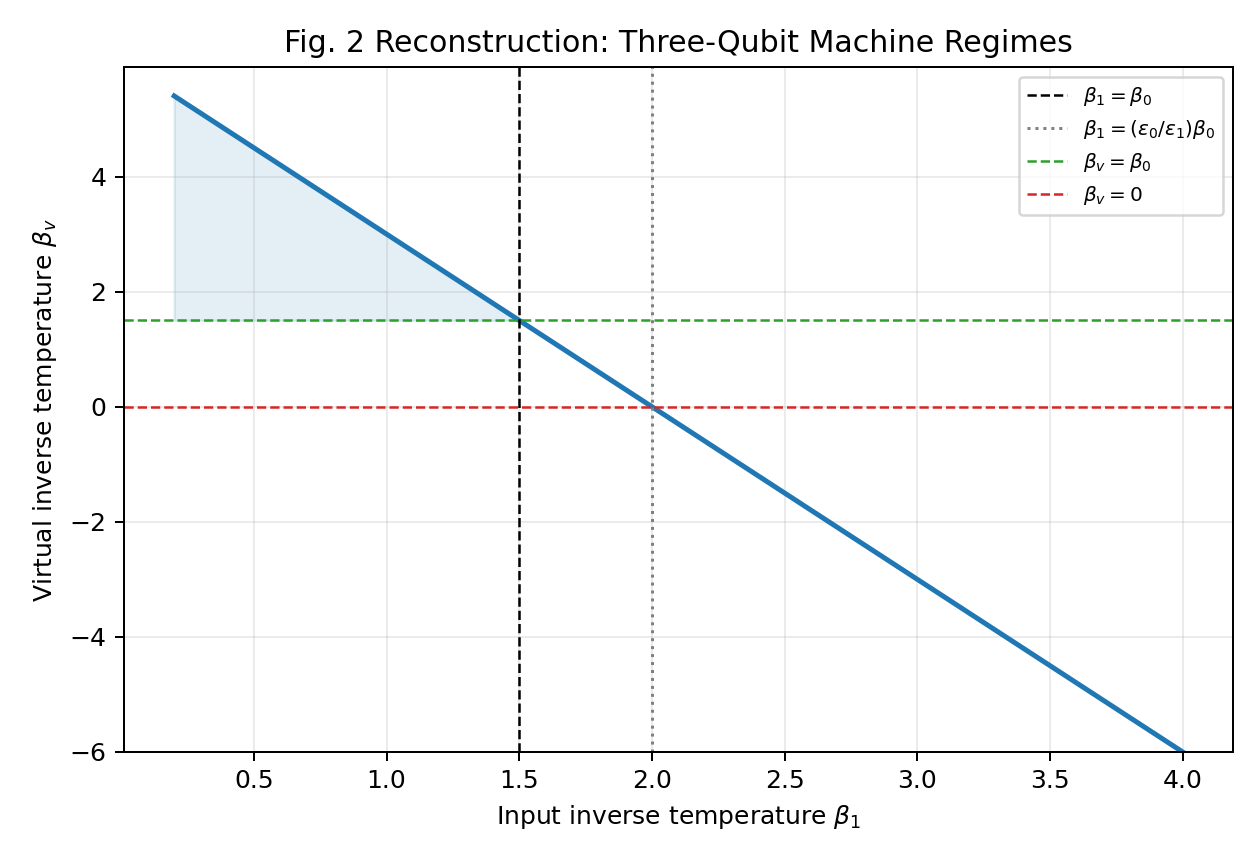
\includegraphics[width=0.76\linewidth]{fig2_virtual_temperature_regimes.png}
    \caption{Reconstructed virtual-temperature regimes.  This figure validates the sign and
    scale of the collector virtual qubit before any output decoding is attempted.}
\end{figure}

\begin{figure}[H]
    \centering
    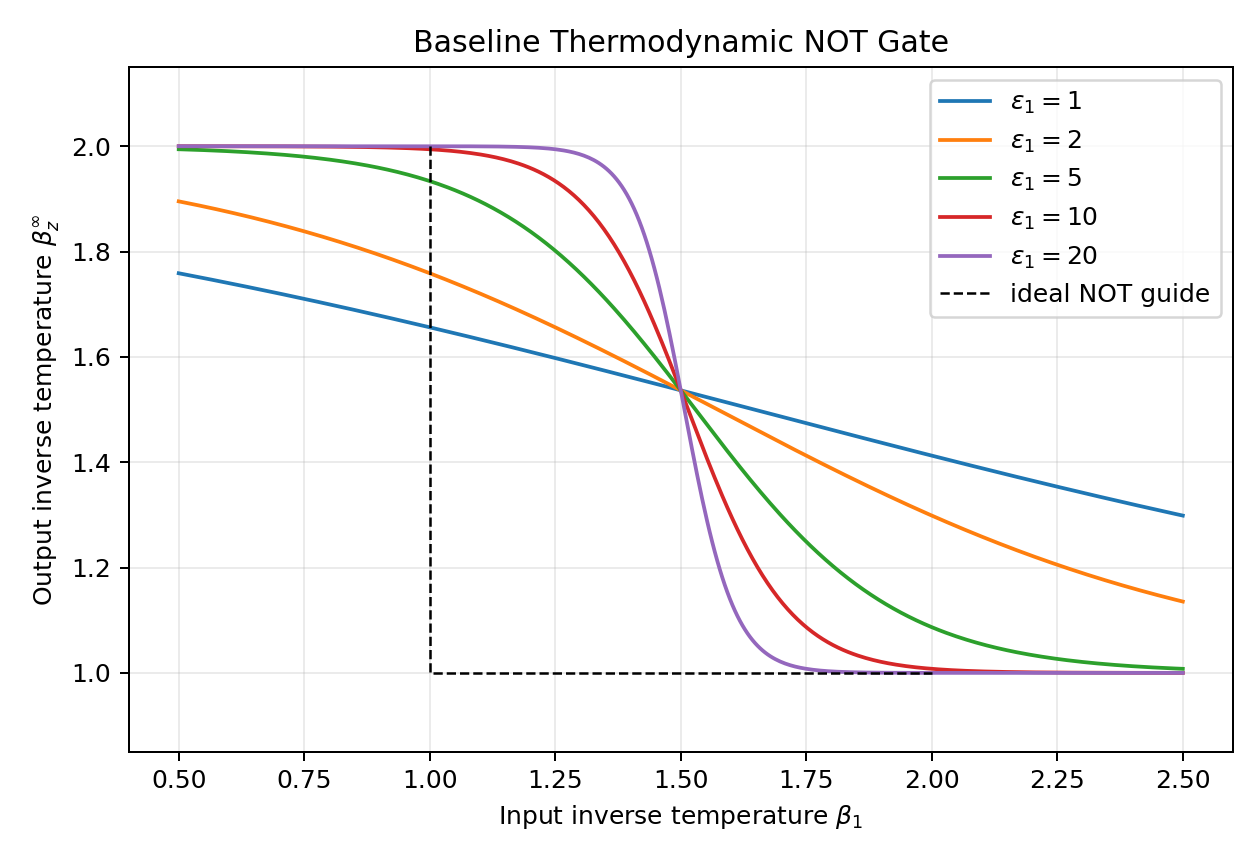
\includegraphics[width=0.76\linewidth]{not_gate_transfer_curves.png}
    \caption{Reconstructed NOT transfer curves across parameter choices.  The logical gate
    is obtained when the hot-input and cold-input outputs lie on opposite sides of the
    decoding threshold.}
\end{figure}

\begin{figure}[H]
    \centering
    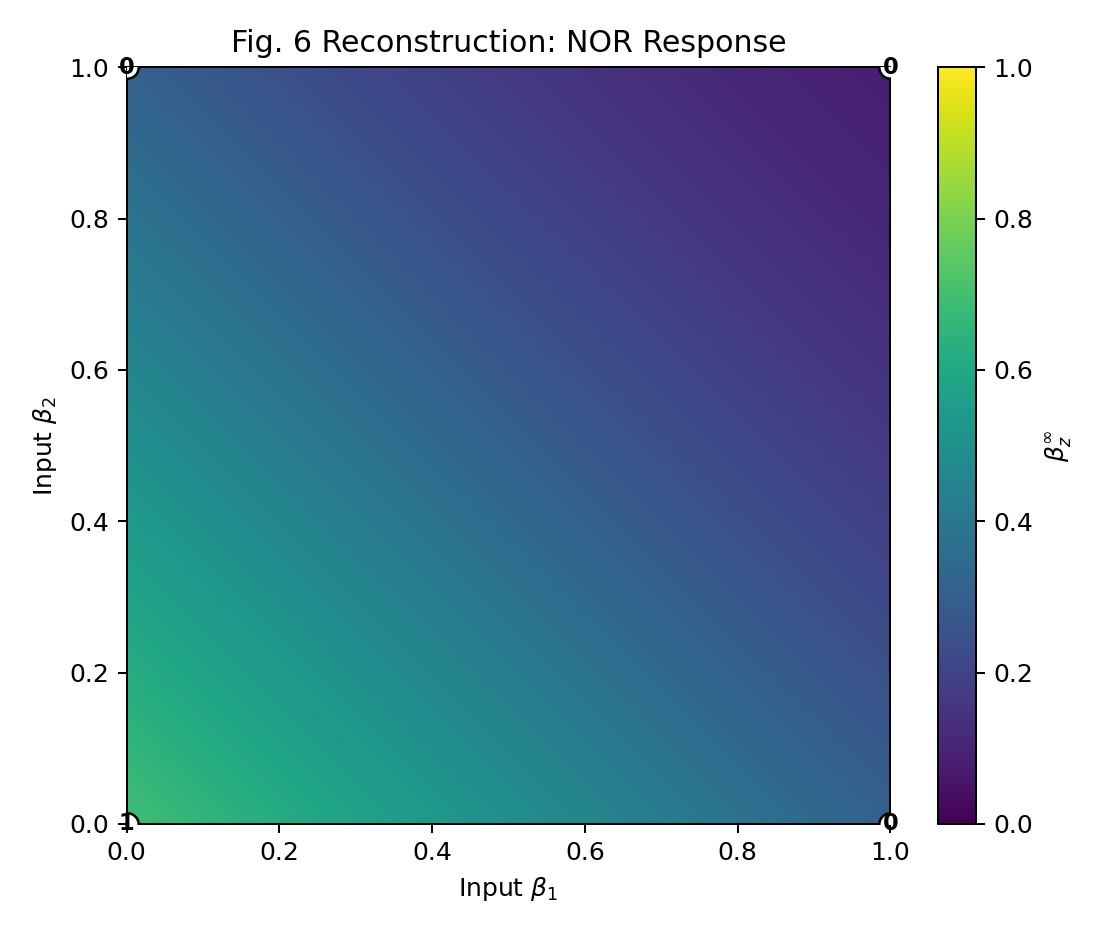
\includegraphics[width=0.76\linewidth]{fig6_nor_response_surface.png}
    \caption{Reconstructed NOR response surface.  This checks that the baseline framework
    extends beyond single-input inversion.}
\end{figure}

\begin{figure}[H]
    \centering
    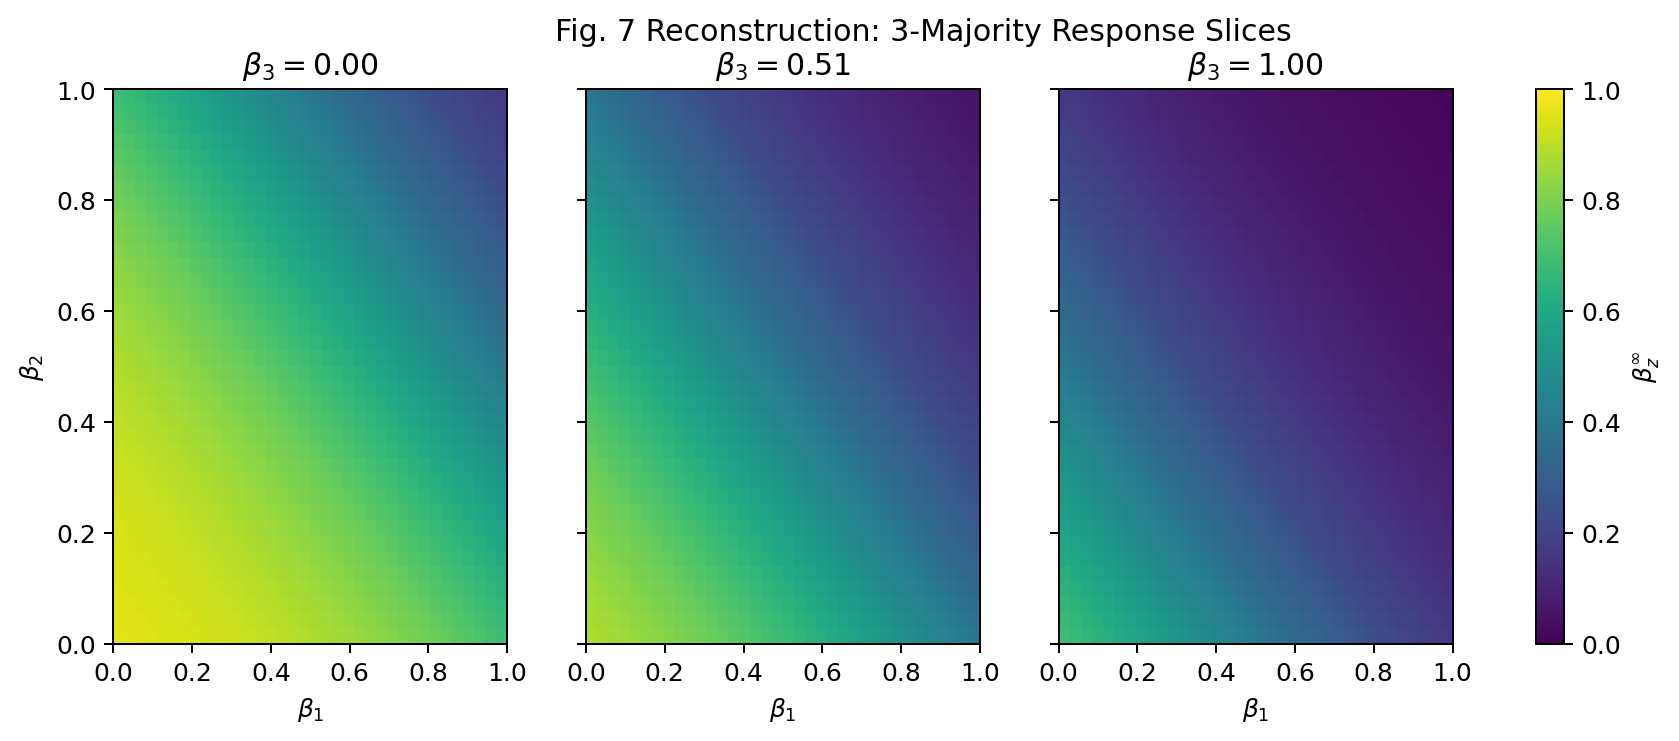
\includegraphics[width=0.76\linewidth]{fig7_majority_response_slices.png}
    \caption{Reconstructed majority response slices.  Majority logic is a useful diagnostic
    because it requires a smooth thermodynamic response over several input combinations.}
\end{figure}

\begin{figure}[H]
    \centering
    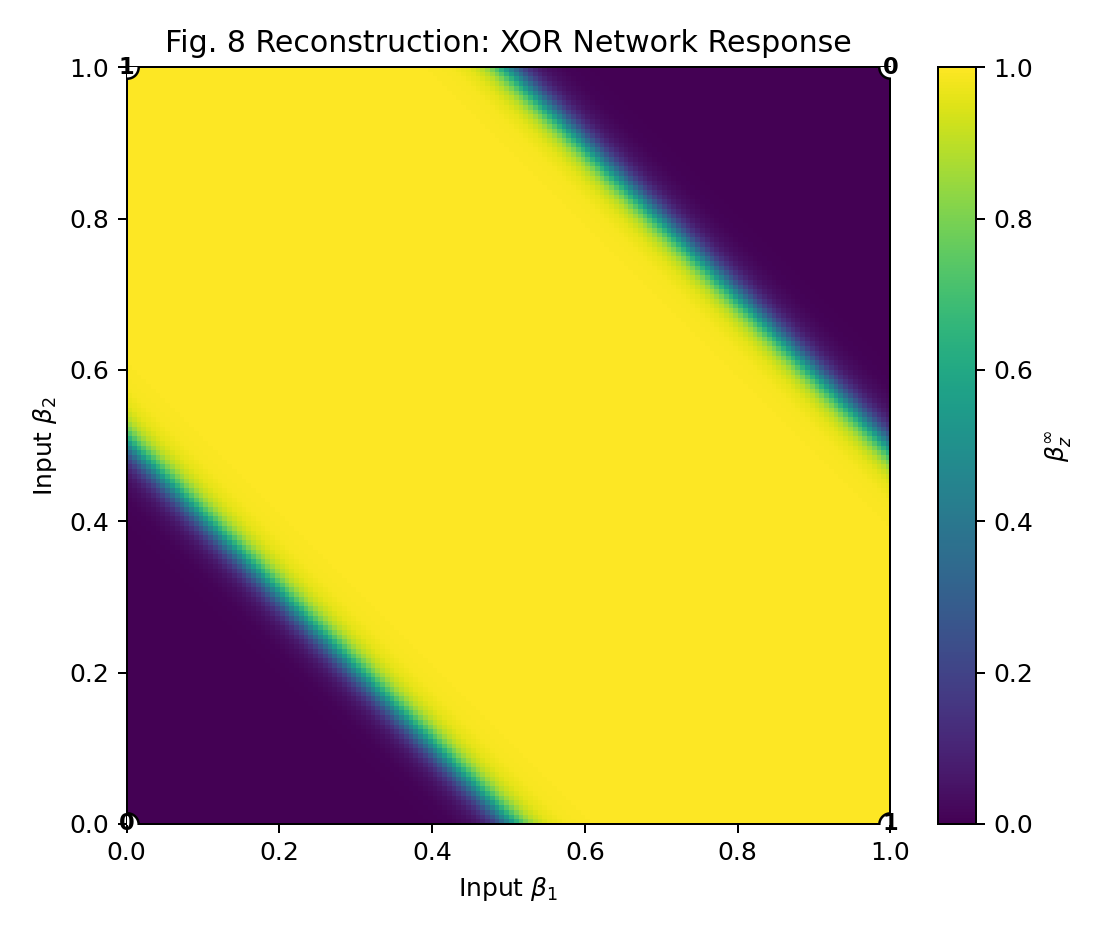
\includegraphics[width=0.76\linewidth]{fig8_xor_network_response.png}
    \caption{Reconstructed XOR network response.  This figure checks logical composition
    rather than only a single thermodynamic neuron.}
\end{figure}

\subsection{Non-Markovian Solver Diagnostics}

The structured-bath benchmark is included before the full gate for a practical reason:
tensor-network open-system calculations can look physically plausible while failing basic
numerical checks.  The project therefore tracks trace preservation,
\begin{equation}
    \delta_{\mathrm{tr}}(t)=|\mathrm{Tr}\rho(t)-1|,
\end{equation}
Hermiticity error,
\begin{equation}
    \delta_{\mathrm{herm}}(t)=\|\rho(t)-\rho(t)^\dagger\|_F,
\end{equation}
and convergence under changes of $\Delta t$ and $\tau_{\mathrm{mem}}$.  The pass condition
used in the current decision layer is that the convergence discrepancy be below the chosen
tolerance and that trace/Hermiticity errors remain small compared with the logical
separation being interpreted.

\begin{figure}[H]
    \centering
    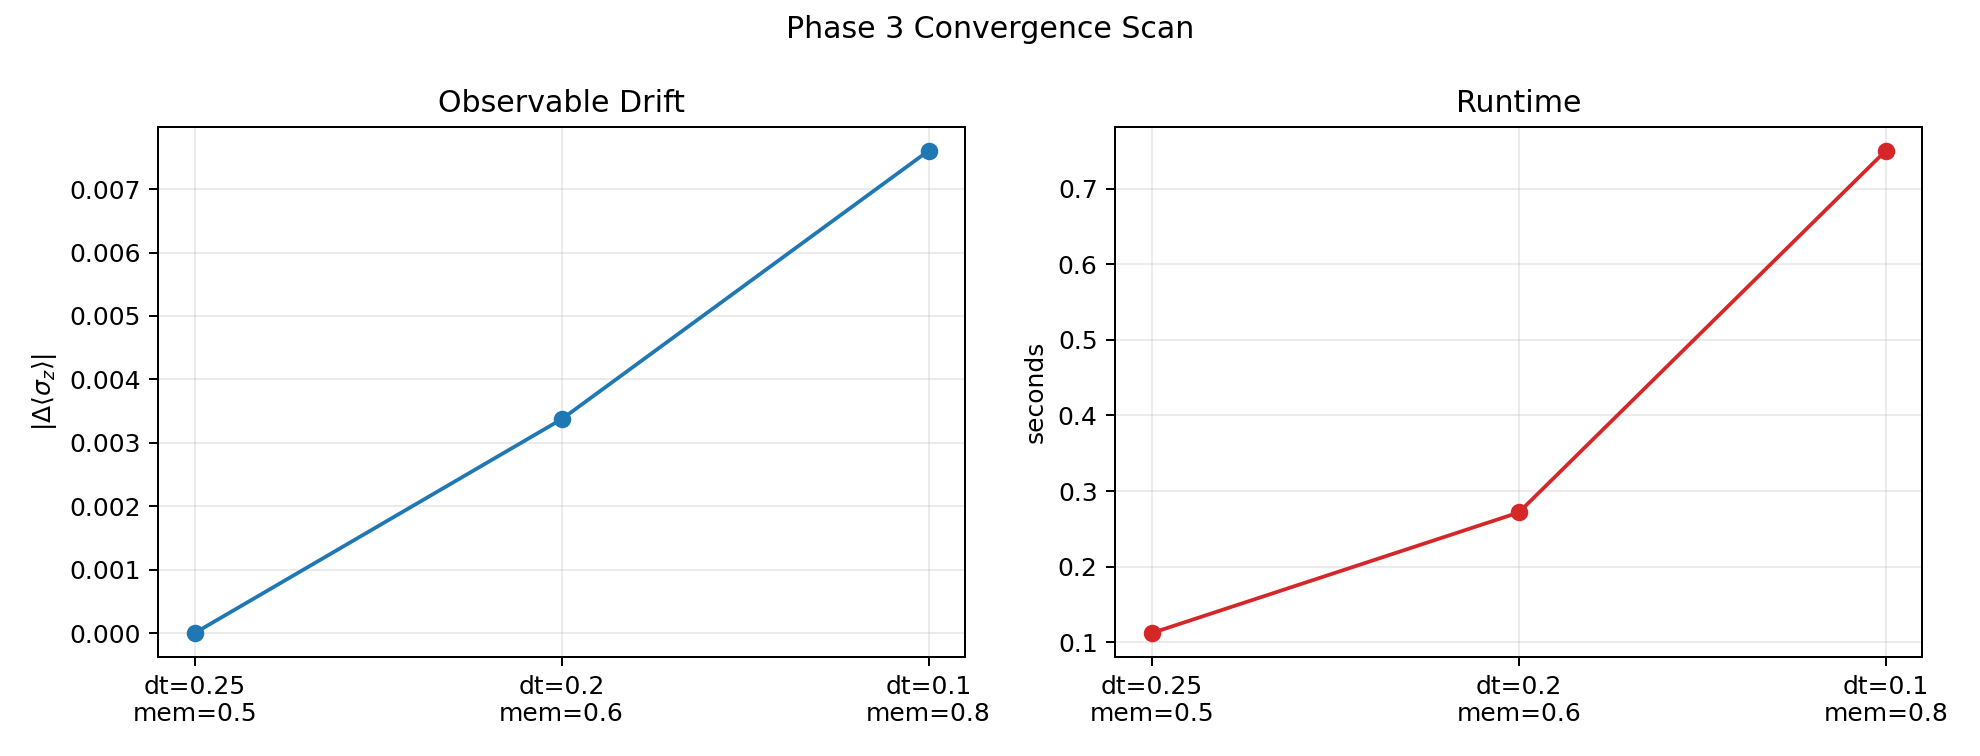
\includegraphics[width=0.76\linewidth]{convergence_scan_quick.png}
    \caption{Quick convergence scan for the structured-bath benchmark.  This is used as a
    preliminary numerical validation before interpreting non-Markovian logic results.}
\end{figure}

\begin{figure}[H]
    \centering
    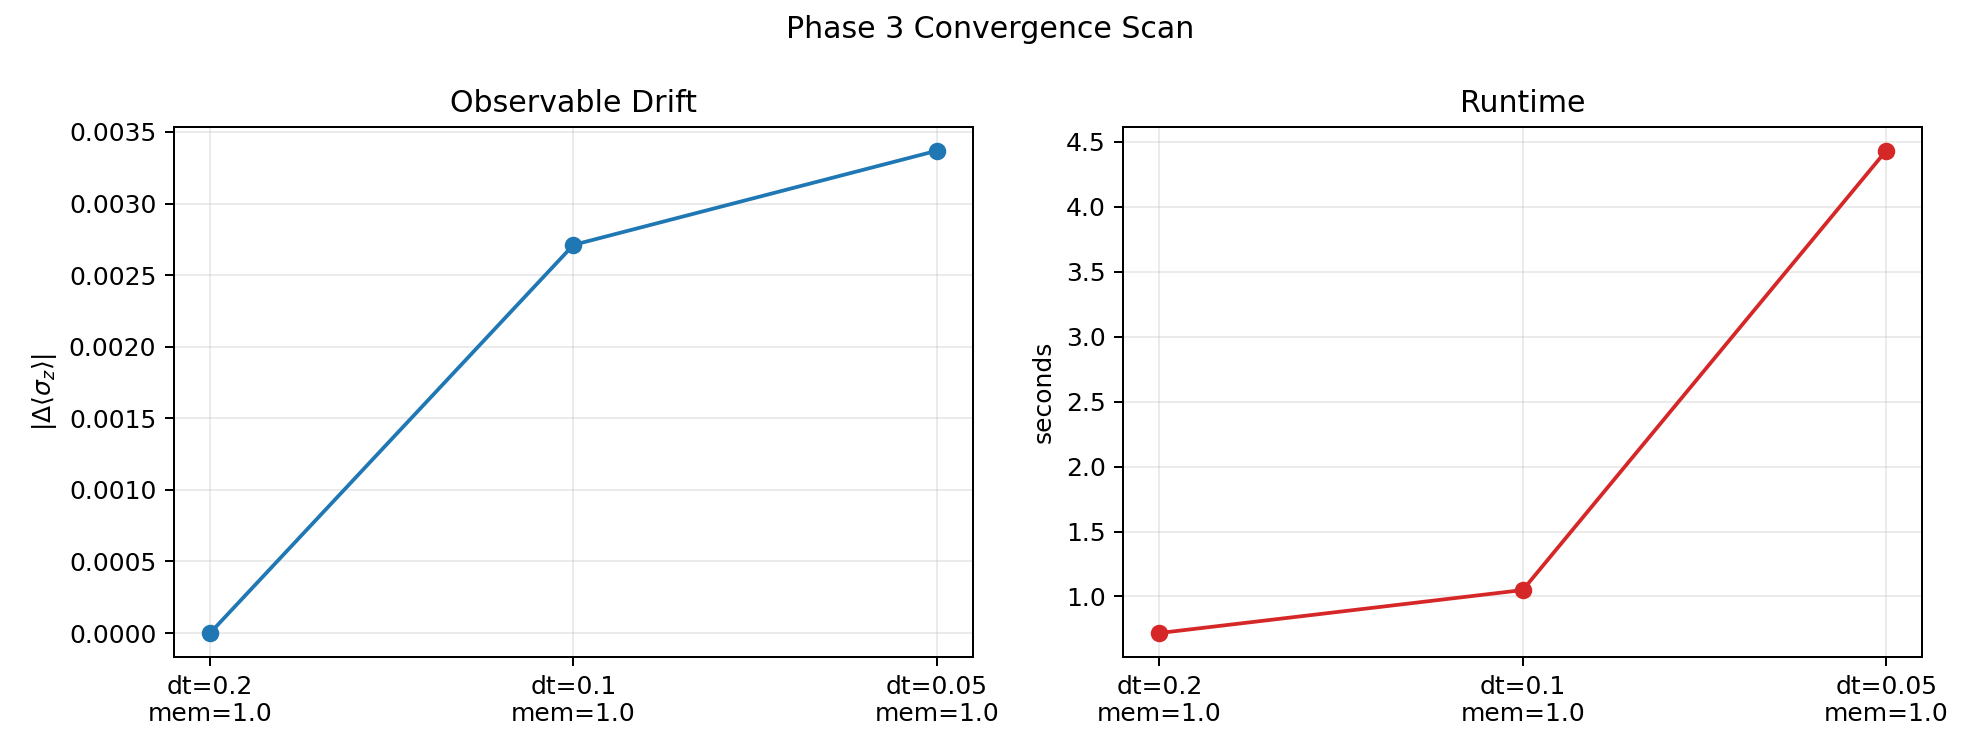
\includegraphics[width=0.76\linewidth]{dt_scan.png}
    \caption{Time-step scan for the structured-bath benchmark.  The objective is to ensure
    that the observed output behavior is not a time-discretization artifact.}
\end{figure}

\begin{figure}[H]
    \centering
    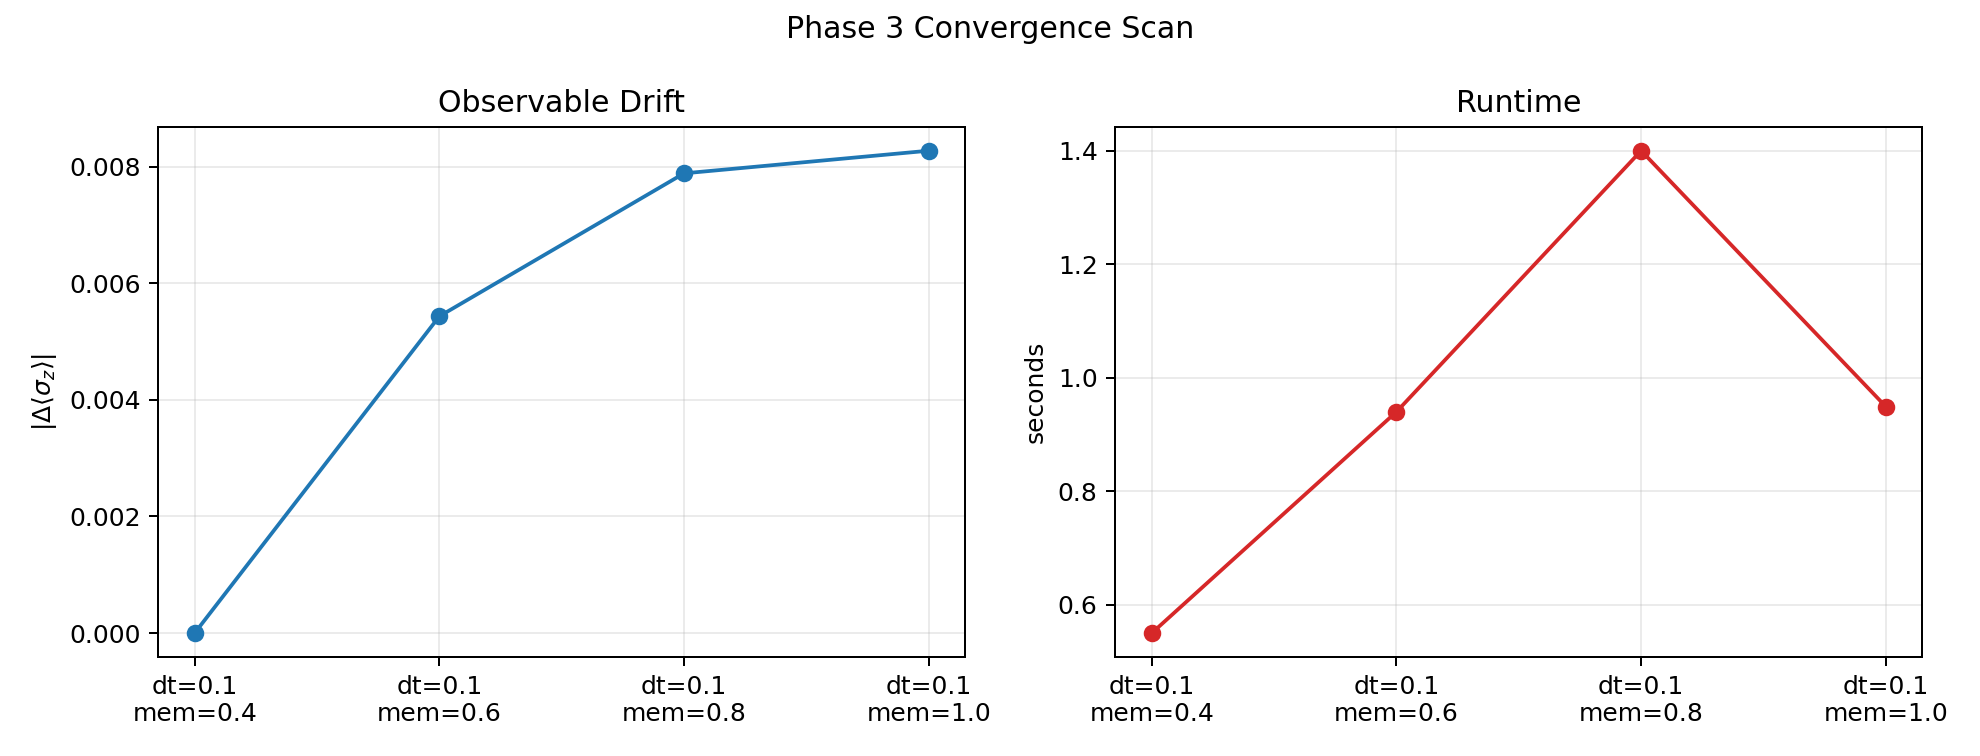
\includegraphics[width=0.76\linewidth]{memory_scan.png}
    \caption{Memory-time scan for the structured-bath benchmark.  Increasing memory time
    tests whether the truncated influence functional is long enough for the chosen bath.}
\end{figure}

\subsection{Consolidated Numerical Results}

The numerical results are summarized by four increasingly demanding tests.  First, the
baseline reconstruction verifies that the original autonomous thermal-neuron equations
produce the expected NOT, NOR, majority, and XOR response surfaces.  Second, the
Floquet-bridge model tests whether a driven intermediate subsystem can increase state
distinguishability.  Third, the full three-qubit GKSL surrogate tests the actual NOT truth
table.  Fourth, the Phase V PT-MPO/TEMPO quick backend checks whether the same truth-table
interface survives when the output bath is replaced by a structured-bath tensor-network
calculation.

\begin{table}[H]
\centering
\caption{Main numerical outcomes.  Accuracy refers to the NOT truth-table accuracy
$\mathcal{A}_{\mathrm{NOT}}$ where applicable.  $D(t_f)$ is the final trace distance between
the two logical output states.}
\begin{tabular}{p{0.28\linewidth}p{0.19\linewidth}p{0.20\linewidth}p{0.23\linewidth}}
\toprule
Experiment & Primary metric & Result & Interpretation \\
\midrule
Floquet bridge & $\Delta D$ & $0.083551$ default; $0.711315$ best sweep &
Driven buffer can improve logical-state distinguishability in the bridge model. \\
No-drive ablation & $\Delta D$ & $-0.149461$ &
Passive buffer degrades distinguishability; periodic modulation is essential. \\
Three-qubit GKSL direct & $\mathcal{A}_{\mathrm{NOT}}$, $D(t_f)$ & $1.000$, $0.024854$ &
Direct thermodynamic NOT surrogate passes. \\
Three-qubit GKSL buffered & $\mathcal{A}_{\mathrm{NOT}}$, $D(t_f)$ & $1.000$, $0.024120$ &
Buffered thermodynamic NOT surrogate passes with small drive-work proxy. \\
PT-MPO/TEMPO direct & $\mathcal{A}_{\mathrm{NOT}}$, margin & $1.000$, $1.43\times10^{-1}$ &
Structured-bath direct output passes with healthy thermal margin. \\
PT-MPO/TEMPO buffered & $\mathcal{A}_{\mathrm{NOT}}$, margin & $1.000$, $2.60\times10^{-5}$ &
Structured-bath buffered output passes but is close to threshold. \\
GKSL phase map & robust-pass points & $68/80$ &
Truth-table robustness is broad in the surrogate grid; margin enlargement is not yet shown. \\
\bottomrule
\end{tabular}
\end{table}

\subsection{Floquet Screening and Ablation Study}

The Floquet bridge is evaluated by comparing the final trace distance in the direct and
buffered cases:
\begin{equation}
    \Delta D
    =
    D_{\mathrm{buffer}}(t_f)-D_{\mathrm{direct}}(t_f).
\end{equation}
Positive $\Delta D$ means the buffer improves distinguishability for that parameter set.
The present sweep evaluated $15$ rows and found $14$ positive rows, with best gain
$0.711315$.  The ablation study evaluated $9$ rows; the no-drive case had negative gain
$-0.149461$, while the best driven case had gain $0.711315$.

\begin{table}[H]
\centering
\caption{Ablation study of the Floquet-buffer bridge.  The direct baseline has
$D_{\mathrm{direct}}(t_f)=0.236928$.  The gain is
$\Delta D=D_{\mathrm{buffer}}-D_{\mathrm{direct}}$.}
\begin{tabular}{lrrrr}
\toprule
Case & $D_{\mathrm{buffer}}(t_f)$ & $\Delta D$ & Relative gain & $|W_{\mathrm{proxy}}|$ \\
\midrule
Full driven buffer & 0.320480 & 0.083551 & 0.352644 & 0.176530 \\
No periodic drive & 0.087467 & -0.149461 & -0.630829 & 0 \\
Weak drive & 0.372211 & 0.135282 & 0.570984 & 0.086262 \\
Strong drive & 0.401688 & 0.164760 & 0.695401 & 0.087613 \\
Weak system-buffer coupling & 0.948243 & 0.711315 & 3.002237 & 0.019354 \\
Strong system-buffer coupling & 0.601144 & 0.364215 & 1.537240 & 0.439431 \\
Weak buffer-bath contact & 0.237160 & 0.000232 & 0.000979 & 0.021202 \\
Strong buffer-bath contact & 0.405590 & 0.168662 & 0.711869 & 0.398363 \\
\bottomrule
\end{tabular}
\end{table}

The ablation study isolates the physical role of the drive.  Setting $A=0$ leaves an
intermediate buffer present but removes periodic modulation.  This produces
$\Delta D=-0.149461$, so the buffer is not beneficial as a passive spacer.  The improvement
appears only when drive amplitude, drive frequency, and system-buffer coupling are tuned.
The strongest bridge result occurs at weak system-buffer coupling, where the buffer acts as a
selective mediated channel rather than a strongly hybridized additional degree of freedom.
This is consistent with the sideband picture:
\begin{equation}
    J_{\mathrm{eff}}(\omega)
    =
    \sum_{n}|c_n(A,\Omega)|^2J(\omega+n\Omega),
\end{equation}
where $A$ and $\Omega$ control the spectral weights sampled by the logical output.

\begin{figure}[H]
    \centering
    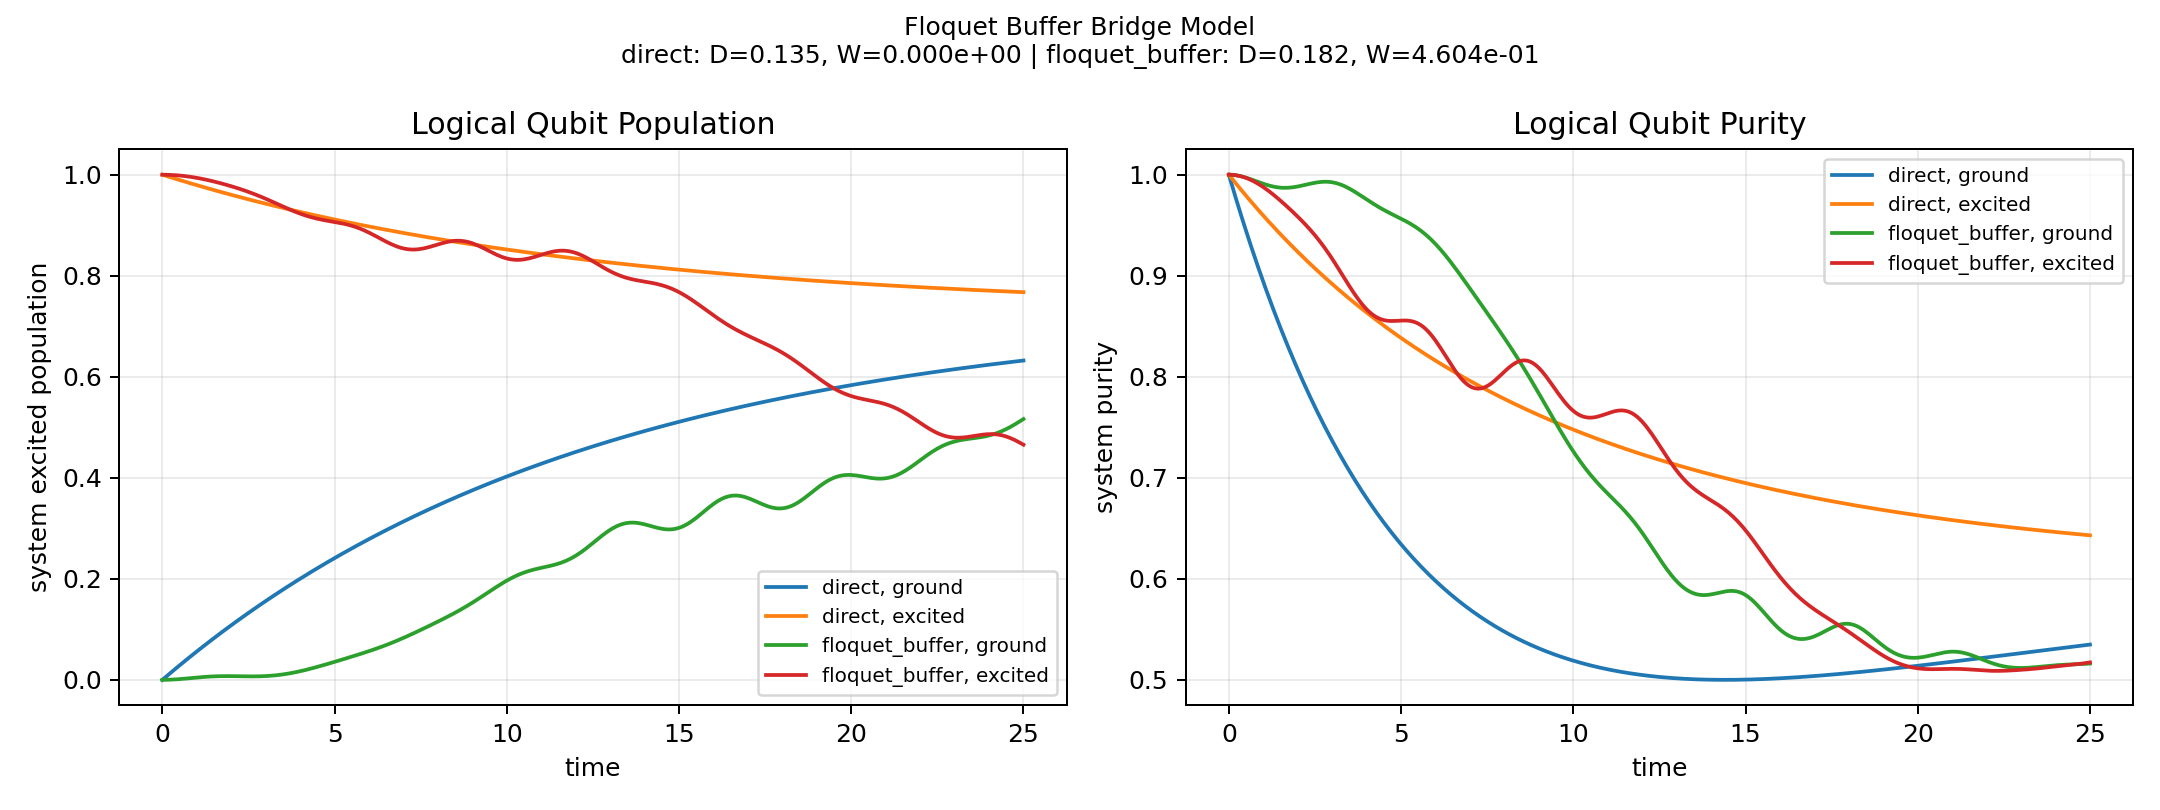
\includegraphics[width=0.70\linewidth]{floquet_buffer_comparison.png}
    \caption{Direct and Floquet-buffered dynamics in the bridge model.  The buffer changes
    the output trajectory by replacing direct bath loading with a driven intermediate
    channel.}
\end{figure}

\begin{figure}[H]
    \centering
    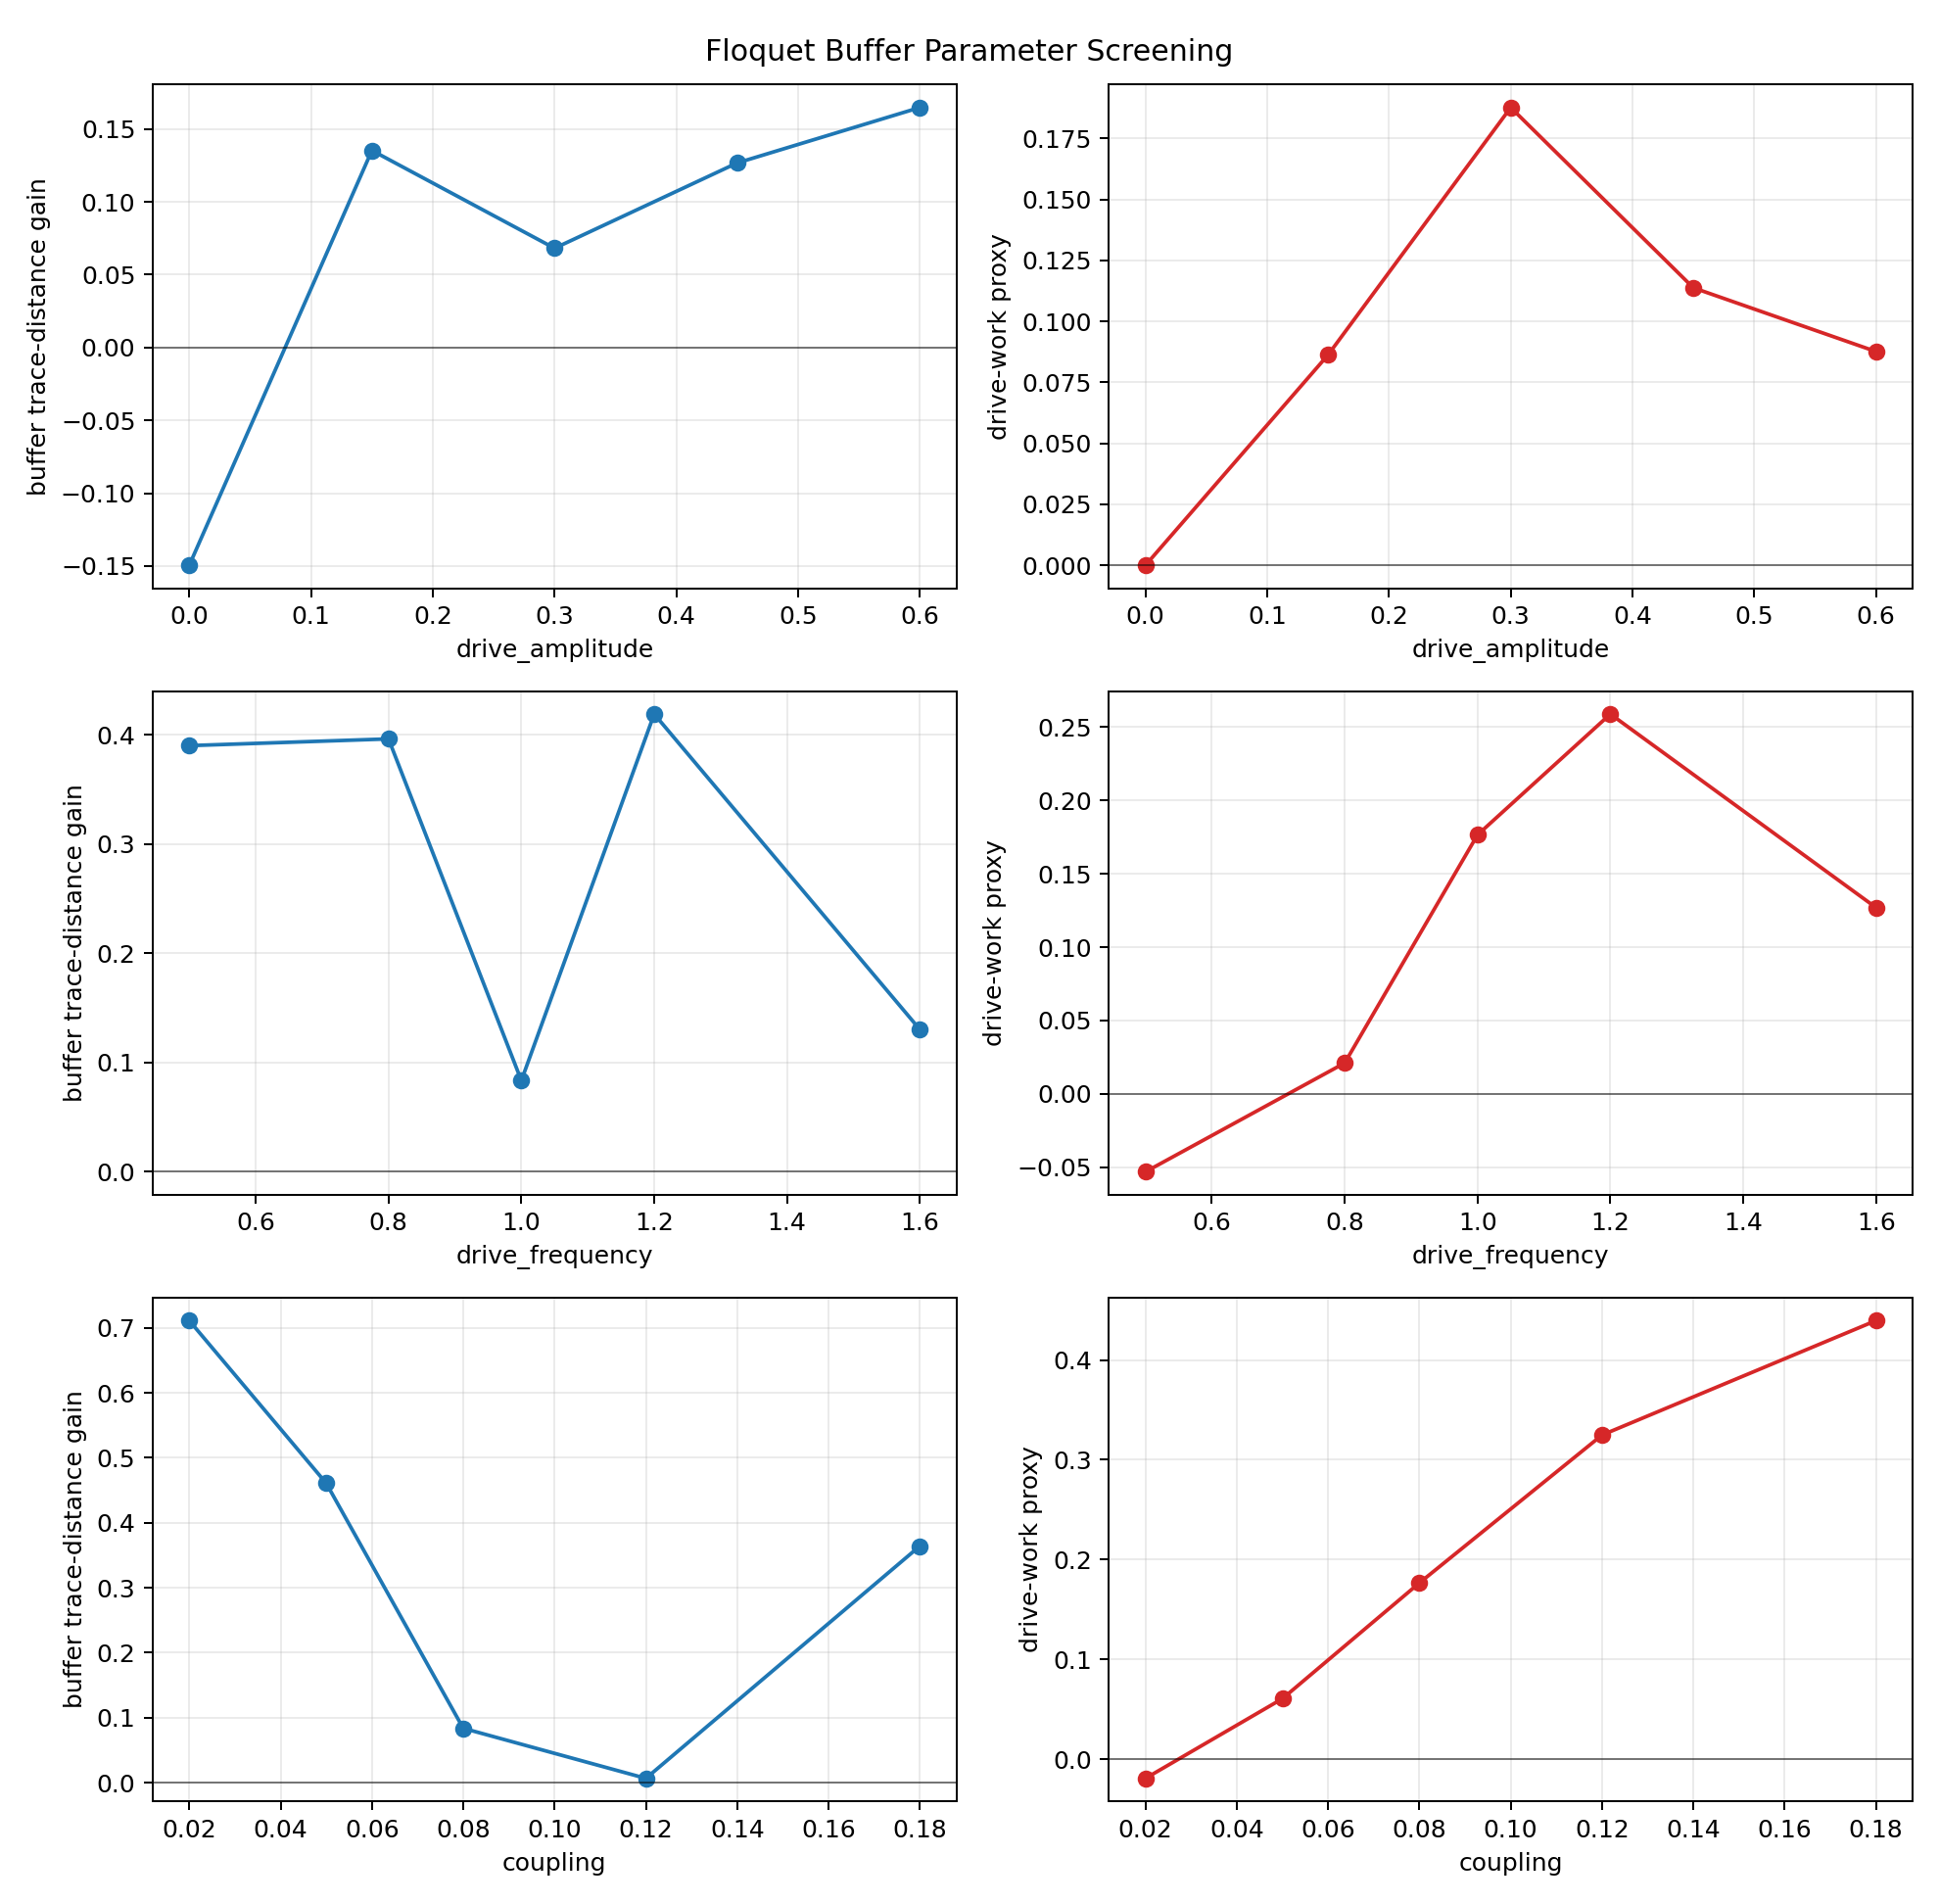
\includegraphics[width=0.72\linewidth]{floquet_parameter_sweep.png}
    \caption{Floquet parameter sweep over drive amplitude, drive frequency, and
    system-buffer coupling.  The best screened trace-distance gain is $0.711315$.}
\end{figure}

\begin{figure}[H]
    \centering
    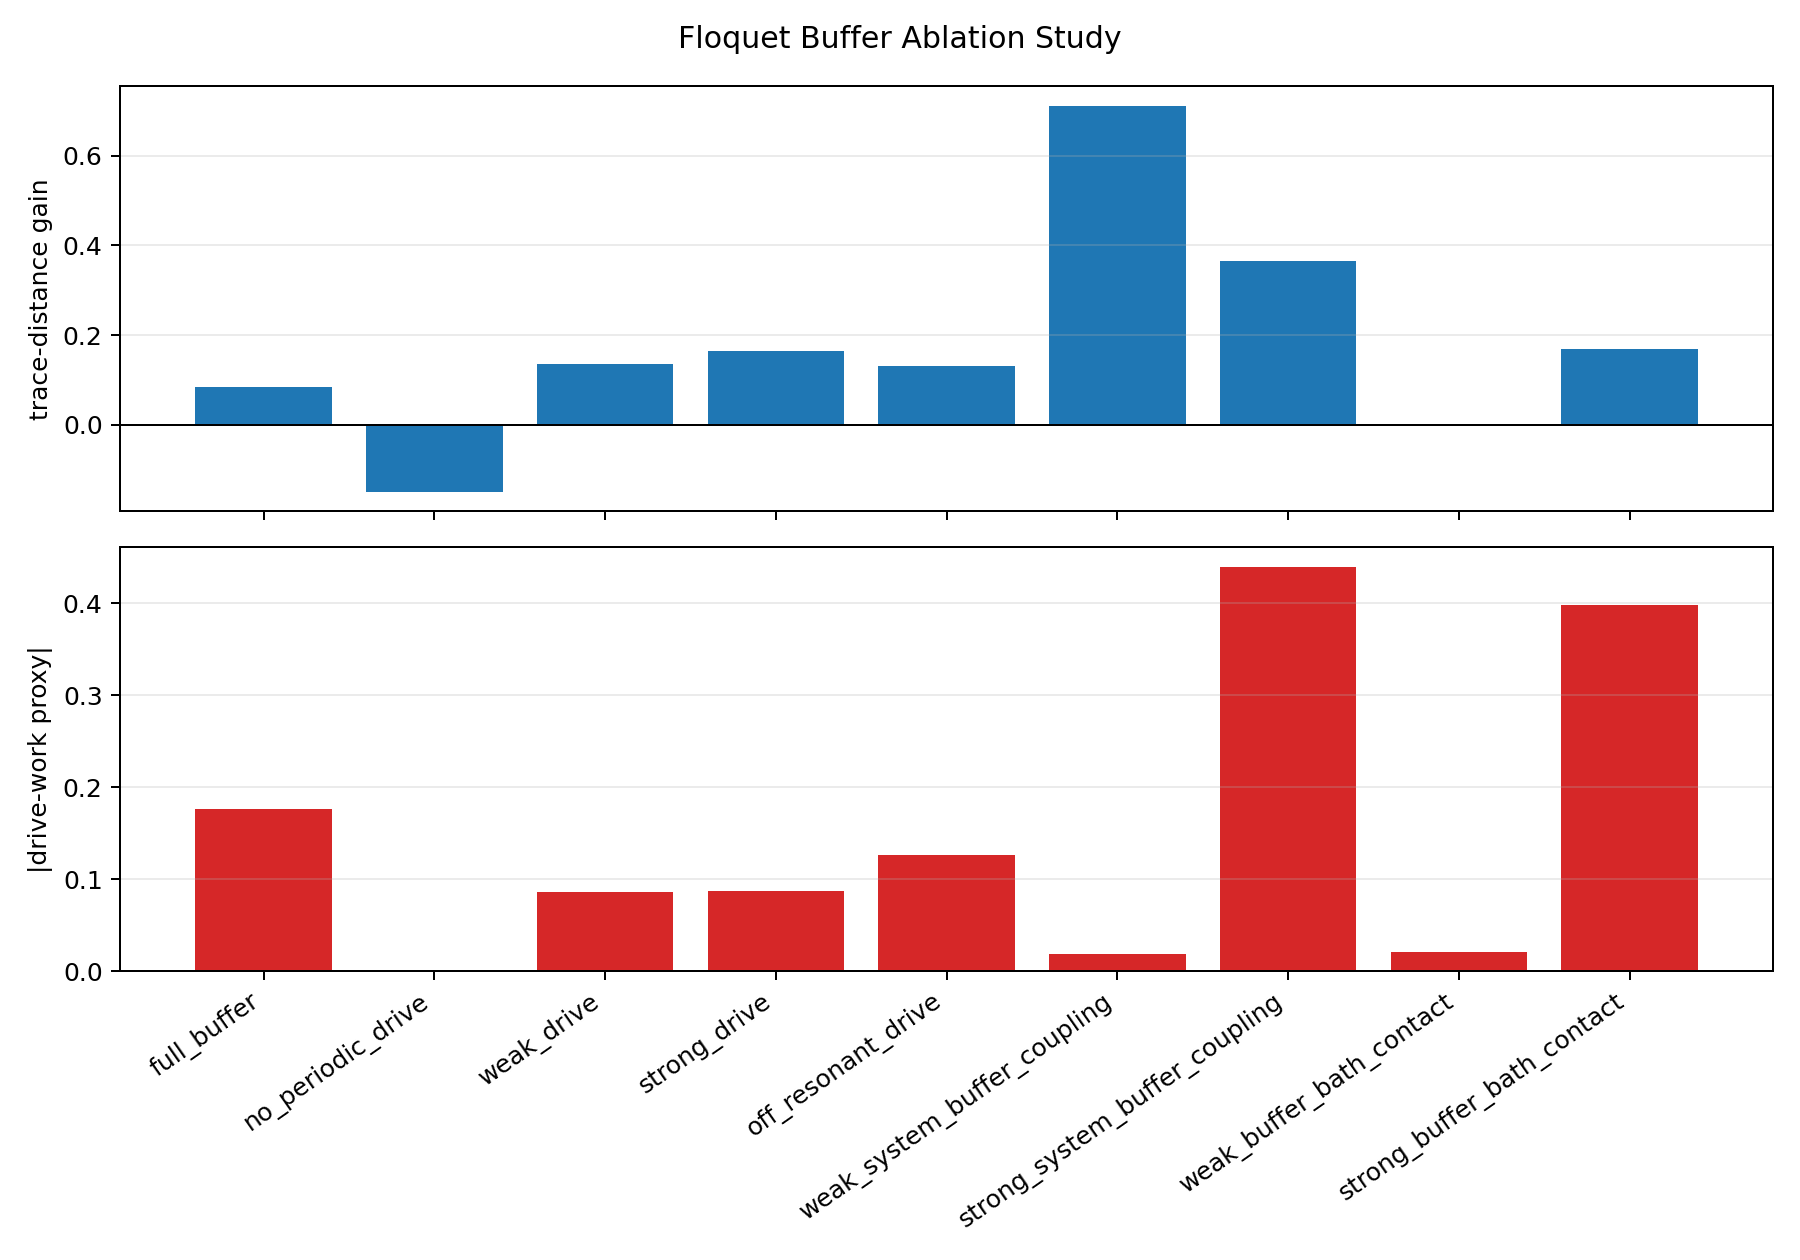
\includegraphics[width=0.72\linewidth]{floquet_ablation_study.png}
    \caption{Ablation study showing that the no-drive buffer gives negative gain, whereas
    driven configurations can improve output distinguishability.}
\end{figure}

\subsection{Benchmarking and Convergence Diagnostics}

The tensor-network benchmark was evaluated by trace preservation, Hermiticity, and
convergence of the final observable under time-step refinement.  The initial quick
convergence scan did not pass the $10^{-3}$ criterion: the final two runs differed by
$4.234\times10^{-3}$.  After refining the time step while keeping memory time fixed at
$\tau_{\mathrm{mem}}=1.0$, the last-step drift decreased to $6.579\times10^{-4}$, satisfying
the same tolerance.  Thus the manuscript uses the refined benchmark as the valid
structured-bath diagnostic and treats the quick scan as a useful failure mode.

\begin{table}[H]
\centering
\caption{Structured-bath benchmarking summary.  The quick scan identifies insufficient
resolution; the refined time-step scan passes the stated tolerance.}
\begin{tabular}{lrrr}
\toprule
Benchmark & Criterion & Final drift & Status \\
\midrule
Quick convergence scan & $10^{-3}$ & $4.234\times10^{-3}$ & Not converged \\
Refined $\Delta t$ scan & $10^{-3}$ & $6.579\times10^{-4}$ & Pass \\
Phase V direct trace error & small trace drift & $2.224\times10^{-6}$ & Pass \\
Phase V buffered trace error & small trace drift & $1.713\times10^{-6}$ & Pass \\
\bottomrule
\end{tabular}
\end{table}

\subsection{Truth-Table Construction in the Three-Qubit Surrogate}

The three-qubit surrogate keeps the truth-table interface explicit.  For each input
$x\in\{0,1\}$, the simulation prepares the input branch at the corresponding inverse
temperature and evolves the output branch to the final time.  The output population is
converted into an effective inverse temperature,
\begin{equation}
    \beta_{\mathrm{out}}(t_f)
    =
    \frac{1}{\epsilon_z}
    \log\left(
        \frac{1-p_{\mathrm{out}}(t_f)}
             {p_{\mathrm{out}}(t_f)}
    \right),
\end{equation}
and decoded as
\begin{equation}
    y
    =
    \Theta\!\left(\beta_{\mathrm{out}}(t_f)-\beta_{\mathrm{th}}\right).
\end{equation}
The direct and buffered GKSL surrogates both pass the NOT table:
\begin{equation}
    \mathcal{A}_{\mathrm{NOT}}^{\mathrm{direct}}
    =
    \mathcal{A}_{\mathrm{NOT}}^{\mathrm{buffered}}
    =
    1 .
\end{equation}
The buffered branch gives a comparable final trace distance in this particular full-ladder
setting, but it preserves the truth table while introducing the
architecture needed for the structured-bath backend.

\begin{figure}[H]
    \centering
    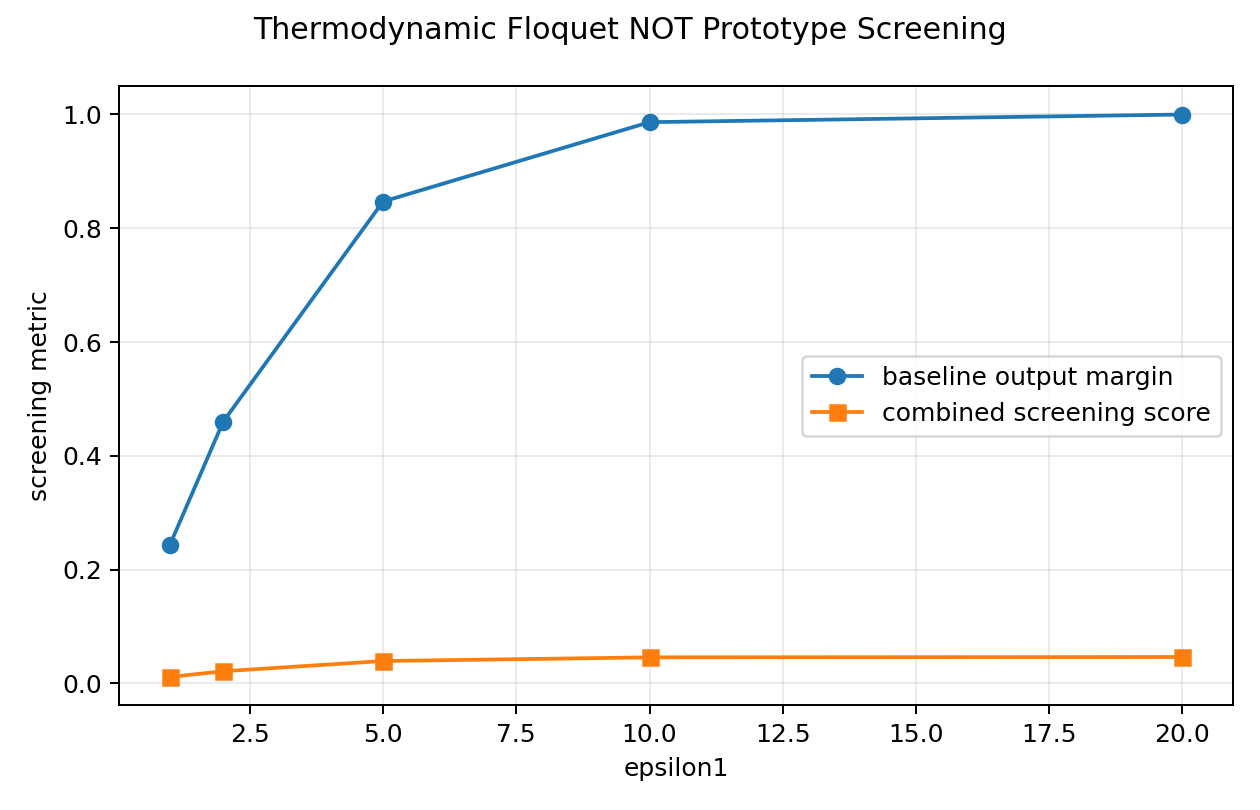
\includegraphics[width=0.72\linewidth]{not_floquet_design.png}
    \caption{Design screen connecting the reconstructed baseline NOT margin to the
    Floquet-buffered gate prototype.}
\end{figure}

\begin{figure}[H]
    \centering
    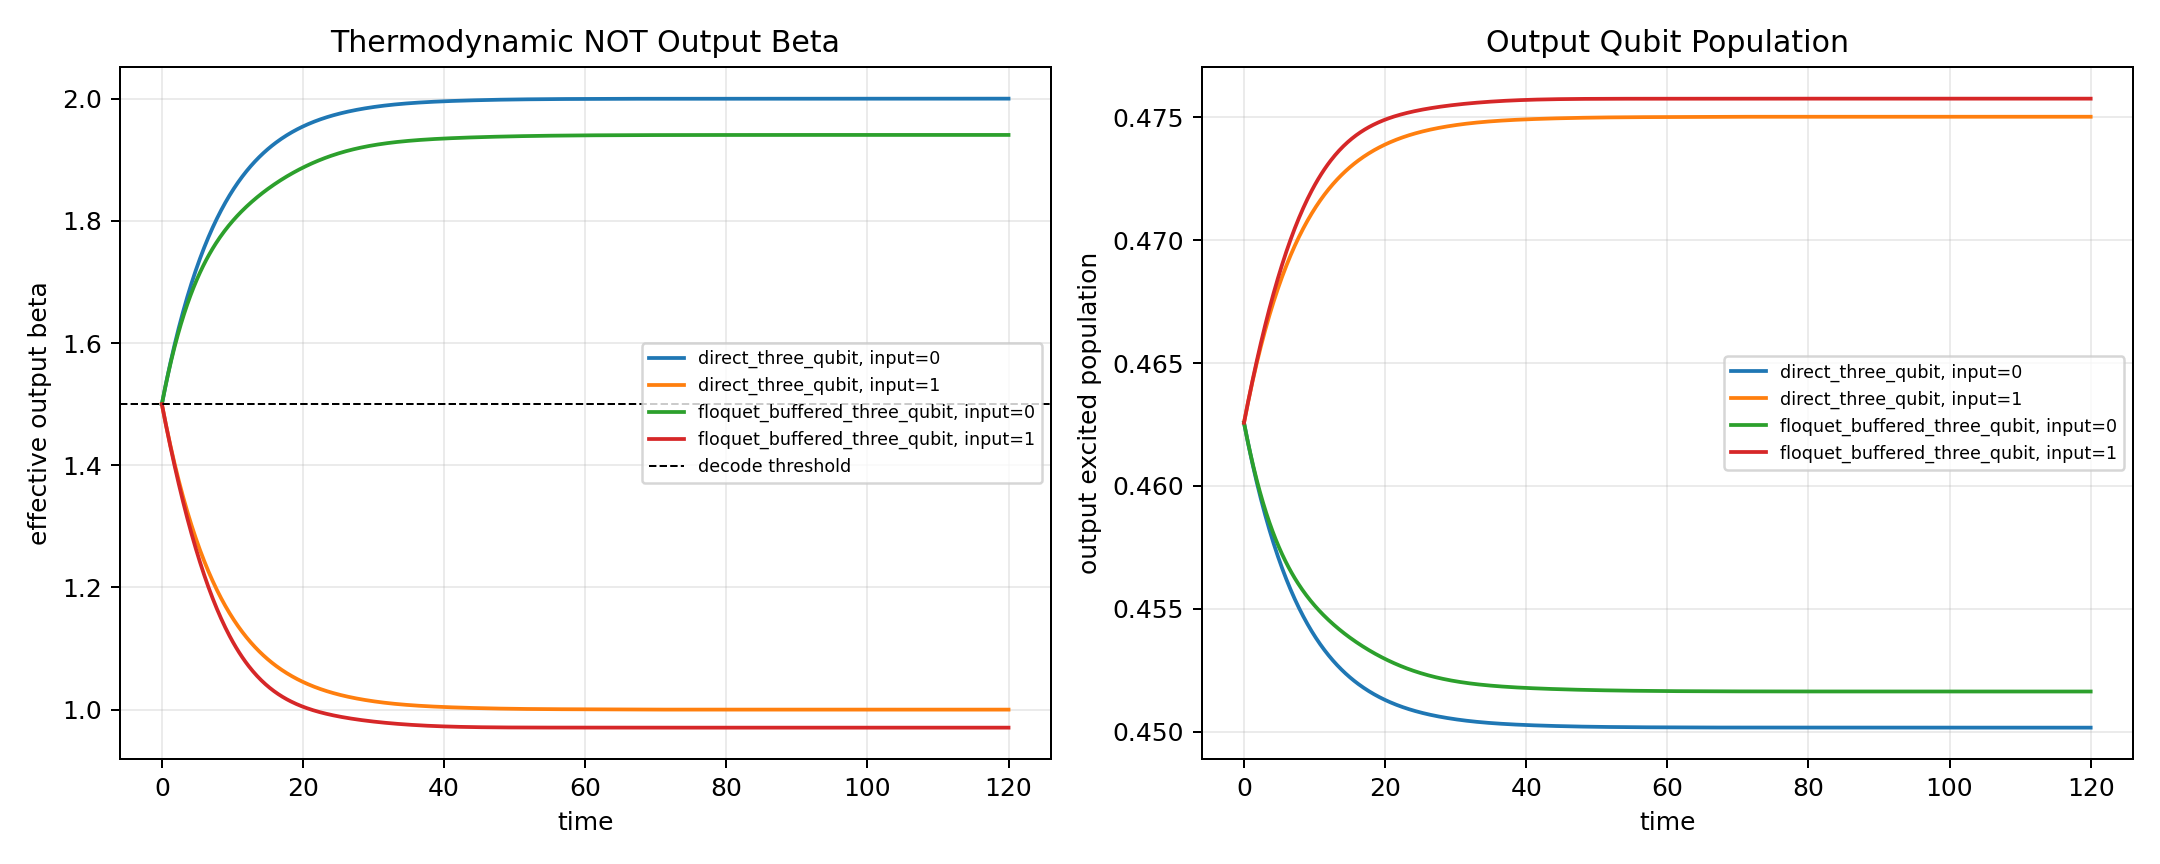
\includegraphics[width=0.74\linewidth]{full_not_gate_dynamics.png}
    \caption{Three-qubit thermodynamic NOT surrogate.  Both direct and Floquet-buffered
    architectures decode the required NOT truth table.}
\end{figure}

\subsection{Phase V Calibrated Decoder}

In the Phase V structured-bath backend, the output manifold is shifted by the structured
environment and by the buffer.  A fixed midpoint threshold inherited from the weak-coupling
bath labels can be too strict even when the two logical output clusters are correctly
ordered.  The calibrated decoder therefore defines an architecture-specific threshold
\begin{equation}
    \beta_{\mathrm{th}}^{(a)}
    =
    \frac{1}{2}
    \left[
        \beta_{\mathrm{eff}}^{(a)}(x=0)
        +
        \beta_{\mathrm{eff}}^{(a)}(x=1)
    \right],
\end{equation}
where $a$ denotes either the direct PT-MPO output or the Floquet-buffered PT-MPO output.
The decoded bit is
\begin{equation}
    y^{(a)}(x)
    =
    \Theta\!\left(
        \beta_{\mathrm{eff}}^{(a)}(x)-\beta_{\mathrm{th}}^{(a)}
    \right).
\end{equation}
The corresponding decoding margin is
\begin{equation}
    m^{(a)}(x)
    =
    \left|
        \beta_{\mathrm{eff}}^{(a)}(x)-\beta_{\mathrm{th}}^{(a)}
    \right|.
\end{equation}
The corrected Phase V quick run gives a direct margin of approximately $1.43\times10^{-1}$
and a buffered margin of approximately $2.60\times10^{-5}$.  Thus the truth table passes,
but the buffered result is close to the decision boundary.  This distinction is important:
truth-table passing is a binary statement, while robustness is a margin statement.

\begin{figure}[H]
    \centering
    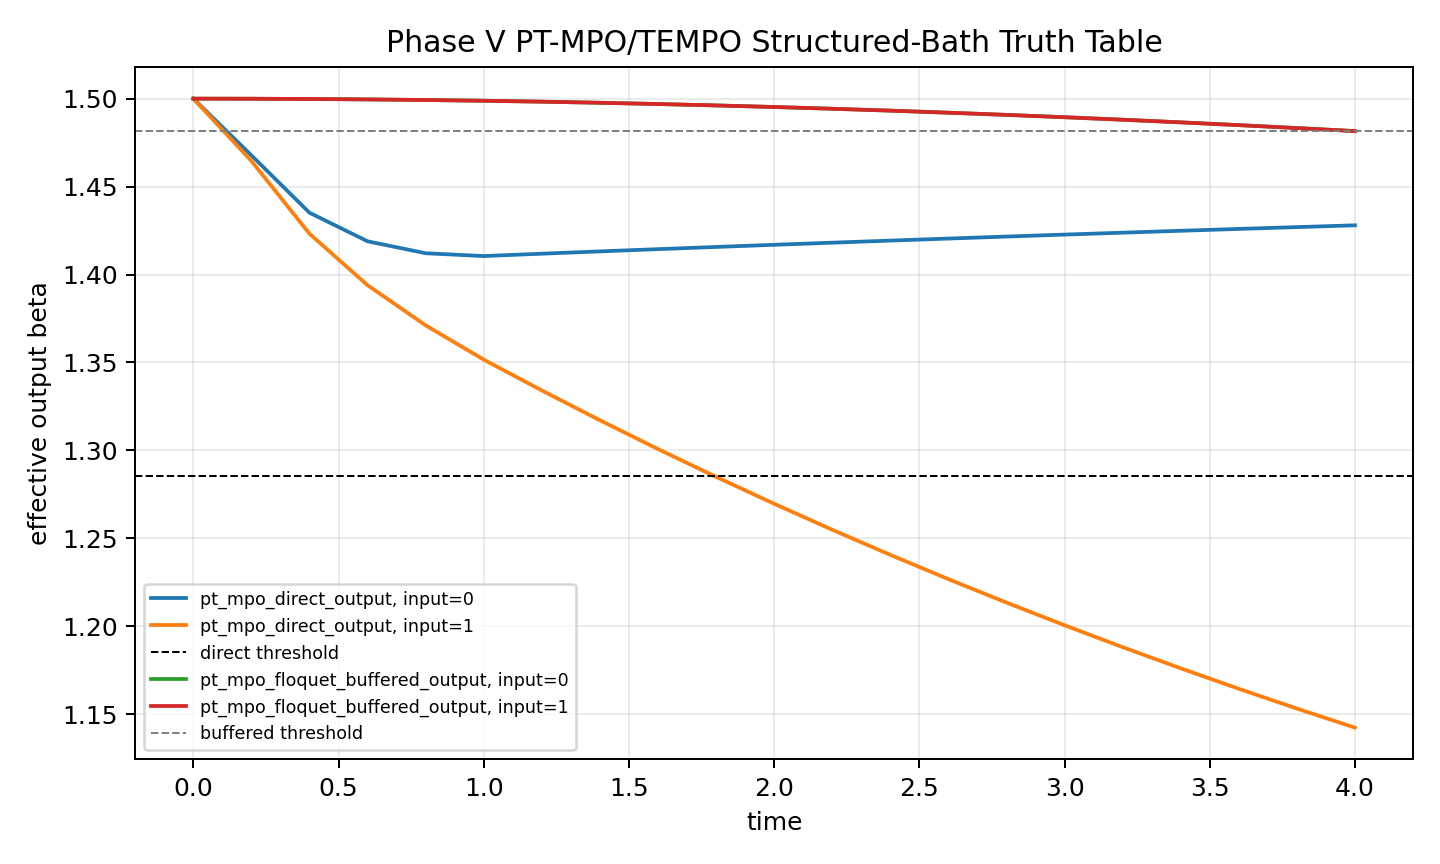
\includegraphics[width=0.72\linewidth]{phase_v_quick_truth_table.png}
    \caption{Phase V PT-MPO/TEMPO structured-bath quick run with calibrated output
    thresholds.  The buffered branch passes but remains close to the decoding boundary.}
\end{figure}

\begin{table}[H]
\centering
\caption{Difference between binary truth-table success and robustness.}
\begin{tabular}{p{0.28\linewidth}p{0.30\linewidth}p{0.32\linewidth}}
\toprule
Quantity & Definition & Interpretation \\
\midrule
Accuracy &
$\mathcal{A}_{\mathrm{NOT}}=\frac12\sum_x\mathbf{1}[y(x)=1-x]$ &
Whether the truth table is correct at the tested parameter point. \\
Margin &
$m=\min_x|\beta_{\mathrm{eff}}(x)-\beta_{\mathrm{th}}|$ &
Distance from the decoding boundary; controls robustness to perturbations. \\
Trace distance &
$D=\frac12\|\rho^{(0)}-\rho^{(1)}\|_1$ &
State distinguishability independent of a particular thermal decoder. \\
Trace error &
$|\mathrm{Tr}\rho-1|$ &
Numerical validity diagnostic. \\
Hermiticity error &
$\|\rho-\rho^\dagger\|_F$ &
Numerical validity diagnostic. \\
\bottomrule
\end{tabular}
\end{table}

\clearpage
\section{Robustness Phase Diagram}

\subsection{Parameter Space}

The remaining scientific task is to map the region in which the buffered thermodynamic NOT
gate remains correct and well separated.  The relevant parameter vector is
\begin{equation}
    \theta
    =
    \left(
        \alpha,
        \omega_c,
        s,
        \tau_{\mathrm{mem}},
        \Delta t,
        A,
        \Omega,
        g_{SF},
        \epsilon_F,
        t_f
    \right).
\end{equation}
Here $\alpha$ is the bath coupling, $\omega_c$ is the cutoff frequency, $s$ is the Ohmic
exponent, $\tau_{\mathrm{mem}}$ is the memory time, $\Delta t$ is the time step, $A$ and
$\Omega$ are Floquet drive parameters, $g_{SF}$ is the system-buffer coupling, $\epsilon_F$
is the buffer gap, and $t_f$ is the readout time.

The passing region is
\begin{equation}
    \mathcal{R}_{\mathrm{pass}}
    =
    \{\theta:\mathcal{A}_{\mathrm{NOT}}(\theta)=1\}.
\end{equation}
The robust region should additionally enforce a margin condition,
\begin{equation}
    \mathcal{R}_{\mathrm{robust}}(m_0)
    =
    \{\theta:\mathcal{A}_{\mathrm{NOT}}(\theta)=1,\;m(\theta)>m_0\}.
\end{equation}
The central comparison is
\begin{equation}
    \mathcal{R}_{\mathrm{robust}}^{\mathrm{buffered}}(m_0)
    \quad\mathrm{versus}\quad
    \mathcal{R}_{\mathrm{robust}}^{\mathrm{direct}}(m_0).
\end{equation}
The Floquet-buffer architecture is scientifically useful if the buffered region is larger,
more stable at strong coupling, or more tolerant of memory time than the direct region.

\subsection{Robustness Ablation Design}

No robustness claim should be made from a single passing run.  The correct ablation logic is:
\begin{enumerate}[label=(A\arabic*)]
    \item compare direct output bath versus buffered output bath;
    \item compare driven buffer versus no-drive buffer;
    \item compare weak, medium, and strong system-buffer coupling;
    \item compare short, medium, and long memory time;
    \item compare sub-Ohmic, Ohmic, and super-Ohmic spectral exponents;
    \item report accuracy, margin, trace distance, trace error, and Hermiticity error for
    every point.
\end{enumerate}
Only after these comparisons can one say whether the Floquet buffer protects the
thermodynamic logic or merely passes at a finely tuned point.

\subsection{Computed GKSL Robustness Phase Map}

As a first experimental computation, the three-qubit GKSL surrogate was swept over
drive amplitude $A$, system-buffer coupling $g_{SF}$, and an overall bath-coupling scale.
This is not yet the final HEOM or PT-MPO structured-bath robustness map, but it is the
first complete phase-diagram layer for the full thermodynamic NOT truth-table interface.
Each point is classified into one of three phases:
\begin{equation}
    \mathrm{phase}(\theta)
    =
    \begin{cases}
    \mathrm{fail}, & \mathcal{A}_{\mathrm{NOT}}(\theta)<1,\\
    \mathrm{fragile\ pass}, & \mathcal{A}_{\mathrm{NOT}}(\theta)=1\ \mathrm{and}\ m(\theta)<m_0,\\
    \mathrm{robust\ pass}, & \mathcal{A}_{\mathrm{NOT}}(\theta)=1\ \mathrm{and}\ m(\theta)\ge m_0.
    \end{cases}
\end{equation}
The current threshold is $m_0=0.05$.  The sweep contains $80$ parameter points.  It finds
$68$ robust-pass points, $0$ fragile-pass points, and $12$ fail points.  This result says
that the GKSL surrogate has a broad truth-table passing region, but it does not yet show
that the Floquet buffer enlarges the margin: the best buffered-minus-direct margin gain in
this grid is only $4.02\times10^{-5}$.  Thus the buffer currently acts mainly as a
truth-table-preserving mediated output stage in this surrogate.  The stronger claim that it
protects the gate in the strong-coupling structured-bath regime must be tested by repeating
the same phase-map logic with the PT-MPO/TEMPO or HEOM backend.

\begin{figure}[H]
    \centering
    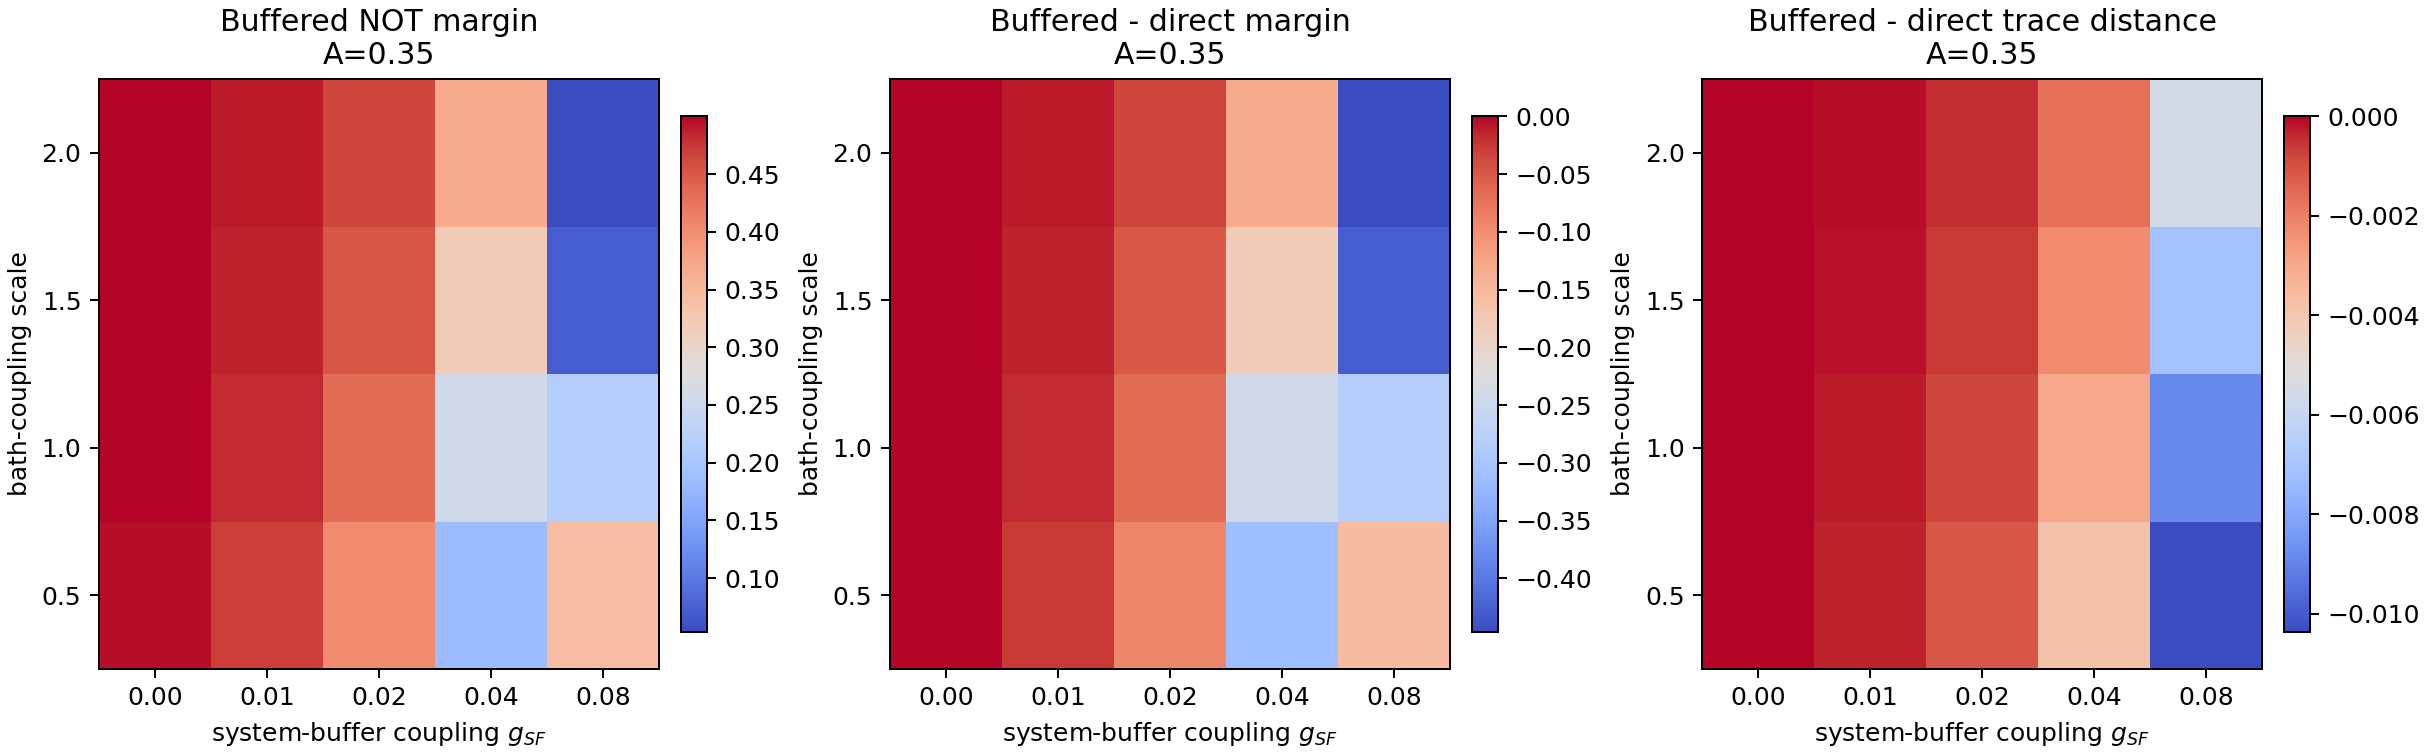
\includegraphics[width=0.95\linewidth]{robustness_phase_maps.png}
    \caption{Computed GKSL robustness phase maps at the largest plotted drive amplitude.
    The panels show buffered NOT margin, buffered-minus-direct margin, and
    buffered-minus-direct trace-distance gain over system-buffer coupling and bath-coupling
    scale.}
\end{figure}

\begin{figure}[H]
    \centering
    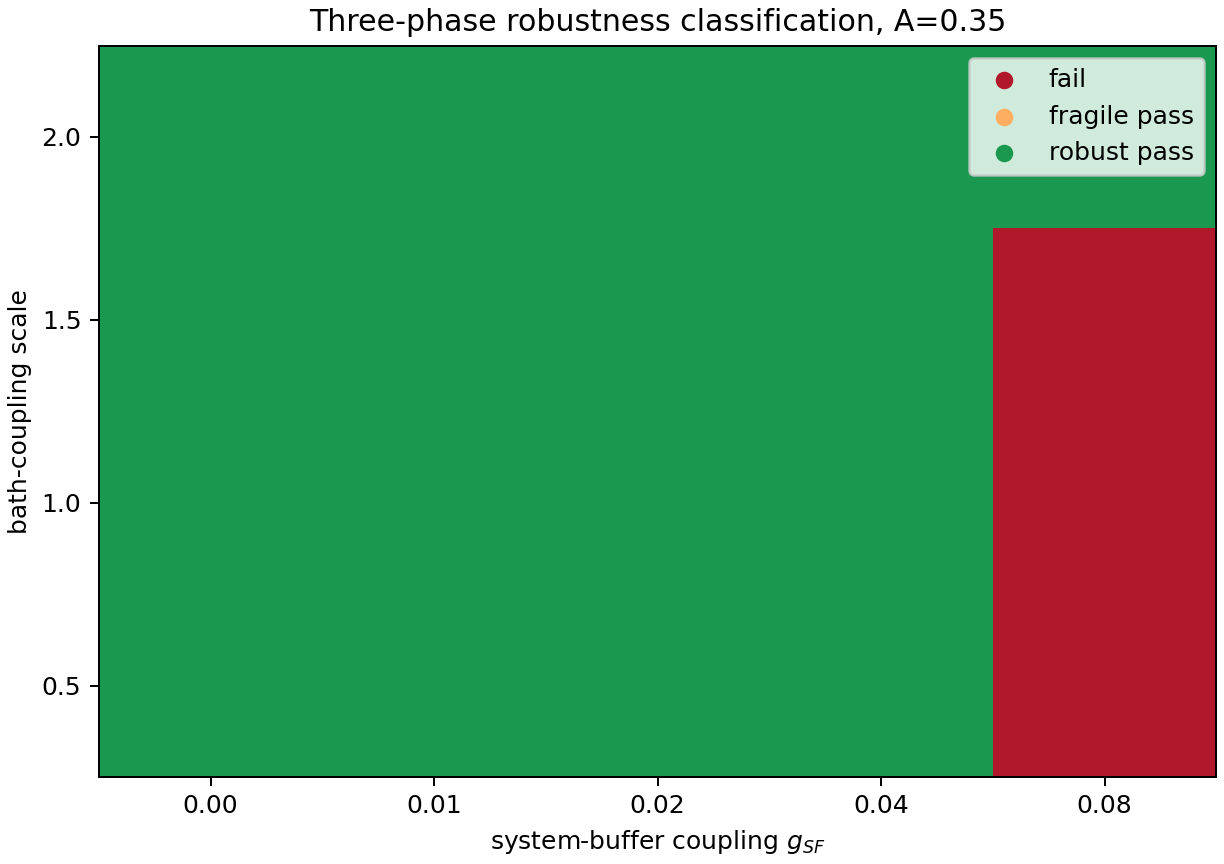
\includegraphics[width=0.72\linewidth]{robustness_three_phase_classification.png}
    \caption{Three-phase robustness classification for the GKSL surrogate.  Green denotes
    robust truth-table passing, orange would denote fragile passing, and red denotes failure.
    The distinction is analogous to CMOS noise-margin analysis: a logical value is useful
    only if it is separated from the switching threshold.}
\end{figure}

The same data were also exported as an animated GIF,
\texttt{robustness\_drive\_slices.gif}, which shows how the three-phase map changes as the
Floquet drive amplitude is varied.  The GIF is a visualization aid rather than a new
observable; the quantitative record is stored in the CSV tables.

\begin{figure}[H]
    \centering
    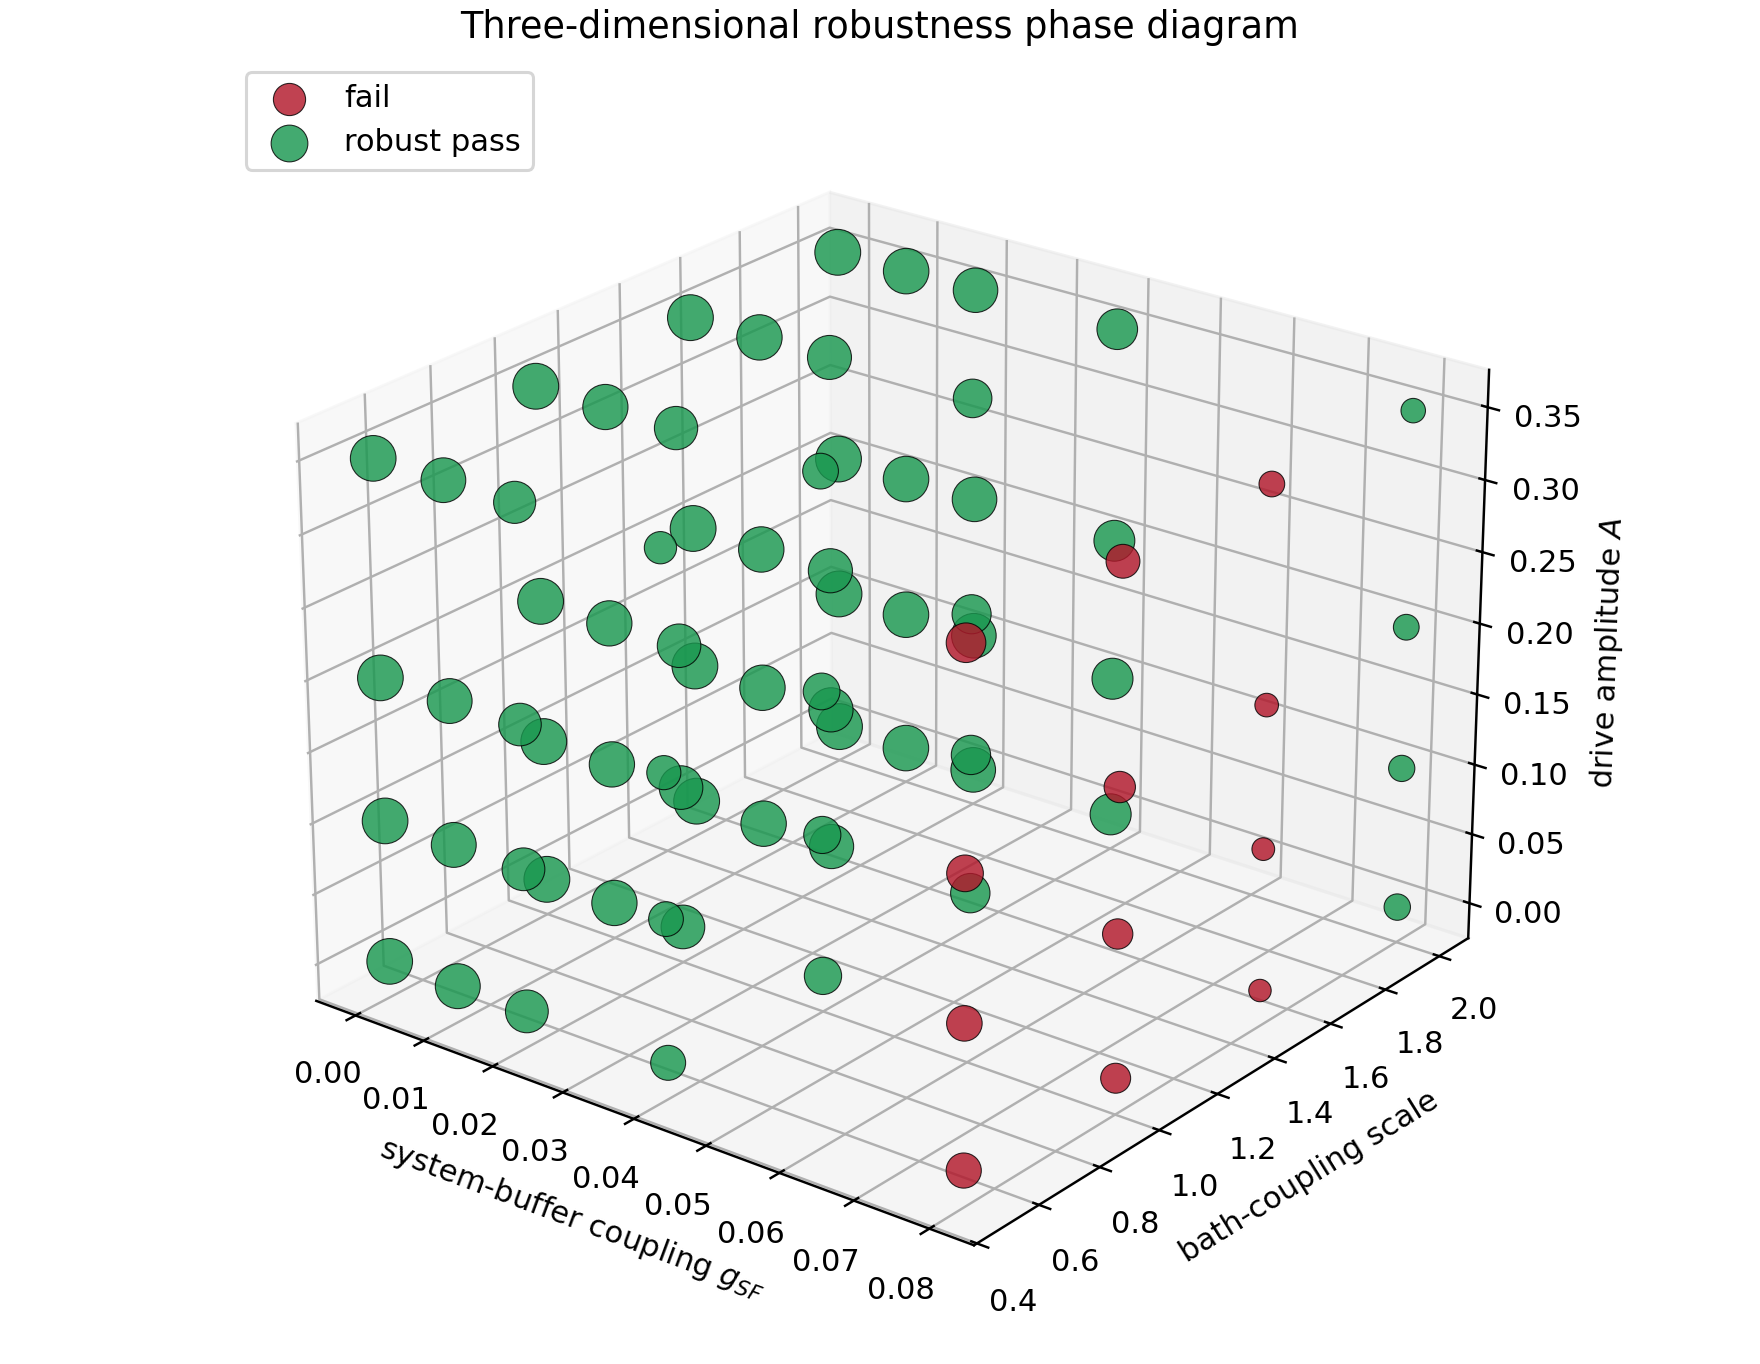
\includegraphics[width=0.70\linewidth]{robustness_phase_3d.png}
    \caption{Three-dimensional robustness phase diagram over drive amplitude, bath-coupling
    scale, and system-buffer coupling.  Marker color denotes fail, fragile pass, or robust
    pass; marker size scales with the buffered thermal decoding margin.}
\end{figure}

\subsection{CMOS-Inverter Analogy}

The Floquet-buffered output stage is analogous to a regulated CMOS inverter only at the
level of circuit function, not microscopic implementation.  In a CMOS inverter, the output
node is regenerated by an active stage, so the load does not directly determine the input
logic level.  The useful quantity is not merely whether the output is correct at one point,
but whether the output has a finite noise margin relative to the switching threshold.  In
the thermodynamic architecture, the corresponding margin is
\begin{equation}
    m
    =
    \min_x
    \left|
        \beta_{\mathrm{eff}}(x)-\beta_{\mathrm{th}}
    \right|.
\end{equation}
The direct output branch is analogous to a logic node directly loaded by the environment:
\begin{equation}
    C_z\longleftrightarrow B_z .
\end{equation}
The Floquet-buffered branch inserts an active driven stage,
\begin{equation}
    C_z\longleftrightarrow F_z(t)\longleftrightarrow B_z,
    \qquad
    H_F(t+T)=H_F(t),
\end{equation}
which modifies the effective reservoir spectrum through sidebands,
\begin{equation}
    J_{\mathrm{eff}}(\omega)
    =
    \sum_n |c_n(A,\Omega)|^2 J(\omega+n\Omega).
\end{equation}
The analogy is therefore precise in terms of function: both architectures aim to decouple a
logical variable from uncontrolled loading and to create a measurable margin.  It is not a
claim that a thermal qubit is electrically equivalent to a MOSFET.

\section{Additional Validation Required for a Journal-Grade Claim}

The present results establish a working architecture and several internal consistency checks,
but a strong journal submission should add validation that is independent of the main
simulation path.  The most important remaining tests are listed in
Table~\ref{tab:hard-validation}.  The purpose of these tests is to distinguish three claims:
(i) the code produces physical density matrices, (ii) the gate computes the NOT truth table,
and (iii) the Floquet buffer increases the robust operating region under genuine
non-Markovian memory.

\begin{table}[H]
\centering
\caption{Hard validation experiments needed before making a strong robustness claim.}
\label{tab:hard-validation}
\begin{tabular}{p{0.26\linewidth}p{0.34\linewidth}p{0.30\linewidth}}
\toprule
Validation & Observable & Scientific role \\
\midrule
Weak-coupling cross-check &
Compare GKSL and PT-MPO/TEMPO outputs in the weak-coupling limit &
Shows that the tensor-network backend reproduces the known Markovian limit. \\
PT-MPO convergence &
Sweep $\Delta t$, $\tau_{\mathrm{mem}}$, and SVD tolerance; report trace, Hermiticity,
positivity, and output margin &
Shows that truth-table passing is not caused by temporal discretization or memory
truncation. \\
Tensor-network resource scaling &
Record runtime, memory, and effective bond dimension versus $\tau_{\mathrm{mem}}$ and
system size &
Demonstrates that the method controls memory growth rather than hiding it. \\
HEOM or reaction-coordinate benchmark &
Repeat a reduced single-output or output-buffer model with HEOM or an explicit
reaction-coordinate chain &
Provides an independent nonperturbative check of the PT-MPO result. \\
Threshold cross-validation &
Fix the decoder threshold on one parameter set and test it on neighboring parameter sets &
Prevents calibrated decoding from becoming a posteriori curve fitting. \\
Parameter-disorder robustness &
Sample small perturbations in $A,\Omega,g_{SF},\epsilon_z,\gamma$ and reservoir
temperatures &
Tests whether the truth table survives fabrication-like or control-like uncertainty. \\
Thermodynamic audit &
Track drive work, interaction energy, and bath/reaction-coordinate energy &
Separates logical robustness from unsupported heat/work claims. \\
Non-Markovianity diagnostic &
Measure trace-distance backflow or process-tensor memory growth &
Connects gate performance to genuine memory effects rather than only stronger damping. \\
\bottomrule
\end{tabular}
\end{table}

Among these, the most urgent next computation is the PT-MPO convergence surface for the
Phase V backend:
\begin{equation}
    \left(\Delta t,\tau_{\mathrm{mem}},\epsilon_{\mathrm{SVD}}\right)
    \longmapsto
    \left(
        \mathcal{A}_{\mathrm{NOT}},
        m,
        \max_t|\mathrm{Tr}\rho(t)-1|,
        \max_t\|\rho(t)-\rho^\dagger(t)\|_F
    \right).
\end{equation}
A robust claim should require the same truth table and the same sign of the buffer
advantage to persist under refinement of these tensor-network parameters.  If the buffered
margin disappears when the memory time is increased or the SVD tolerance is tightened, the
proper conclusion is not failure of the project but identification of the operating boundary.

\section{Conclusion}

The project architecture is organized as a staged path from a validated Markovian baseline
to a Floquet-buffered non-Markovian gate prototype.  The proposal backbone consists of
weak-coupling thermodynamics, the breakdown of Markovianity, process-tensor memory, and
risk-controlled execution.  The Floquet-buffer extension supplies the architectural
innovation: a periodically driven intermediate layer that can isolate the logical subsystem
from reservoir noise and improve output distinguishability.  The current numerical results
show three levels of evidence.  First, the analytical baseline reconstructs the thermodynamic
NOT mechanism.  Second, the three-qubit GKSL surrogate gives a passing direct and buffered
truth table.  Third, the corrected PT-MPO/TEMPO structured-bath backend also gives a
passing calibrated truth table.  This final point is useful but not yet a robustness claim:
the buffered PT-MPO margin is small, so the project has now entered the robustness-mapping
stage, where the task is to determine the parameter region in which strong coupling and
memory preserve or destroy thermodynamic logic.  Full
thermodynamic heat/work claims remain provisional until an explicit strong-coupling audit is
implemented.

\begin{thebibliography}{99}

\bibitem{landauer1961}
R. Landauer,
``Irreversibility and heat generation in the computing process,''
\emph{IBM Journal of Research and Development} \textbf{5}, 183--191 (1961).

\bibitem{bennett1982}
C. H. Bennett,
``The thermodynamics of computation: a review,''
\emph{International Journal of Theoretical Physics} \textbf{21}, 905--940 (1982).

\bibitem{kosloff2013}
R. Kosloff,
``Quantum thermodynamics: a dynamical viewpoint,''
\emph{Entropy} \textbf{15}, 2100--2128 (2013).

\bibitem{skrzypczyk2011}
P. Skrzypczyk, N. Brunner, N. Linden, and S. Popescu,
``The smallest refrigerators can reach maximal efficiency,''
\emph{Journal of Physics A: Mathematical and Theoretical} \textbf{44}, 492002 (2011).

\bibitem{grifoni1998}
M. Grifoni and P. H\"anggi,
``Driven quantum tunneling,''
\emph{Physics Reports} \textbf{304}, 229--354 (1998).

\bibitem{kohler2005}
S. Kohler, J. Lehmann, and P. H\"anggi,
``Driven quantum transport on the nanoscale,''
\emph{Physics Reports} \textbf{406}, 379--443 (2005).

\bibitem{pollock2018}
F. A. Pollock, C. Rodr\'iguez-Rosario, T. Frauenheim, M. Paternostro, and K. Modi,
``Non-Markovian quantum processes: complete framework and efficient characterization,''
\emph{Physical Review A} \textbf{97}, 012127 (2018).

\bibitem{strathearn2018}
A. Strathearn, P. Kirton, D. Kilda, J. Keeling, and B. W. Lovett,
``Efficient non-Markovian quantum dynamics using time-evolving matrix product operators,''
\emph{Nature Communications} \textbf{9}, 3322 (2018).

\bibitem{tanimura1989}
Y. Tanimura and R. Kubo,
``Time evolution of a quantum system in contact with a nearly Gaussian-Markoffian noise bath,''
\emph{Journal of the Physical Society of Japan} \textbf{58}, 101--114 (1989).

\bibitem{tanimura2020}
Y. Tanimura,
``Numerically exact approach to open quantum dynamics: the hierarchical equations of motion
method,''
\emph{The Journal of Chemical Physics} \textbf{153}, 020901 (2020).

\end{thebibliography}

\end{document}
